\chapter{面向车载信息物理融合系统的质量-开销均衡优化策略研究}

本章主要研究面向车载信息物理融合系统的质量-开销均衡优化策略。
具体内容安排如下:\ref{section 5-1} 节是本章的引言,介绍车联网中车载信息物理融合系统的研究现状及存在的不足,同时阐述本章的主要贡献。
接着,在\ref{section 5-2} 节中,将阐述本章的系统架构设计。
在此基础上,\ref{section 5-3} 节给出了系统模型的详细描述。
并在\ref{section 5-4} 节中,形式化定义了一个关于系统中的质量-开销均衡的双目标优化问题。
为解决该问题,\ref{section 5-5} 节设计了一种基于多目标强化学习的优化算法。
为验证所提算法的性能,\ref{section 5-6} 节搭建了实验模拟环境并进行了性能验证。
最后,\ref{section 5-7} 节对本章的研究工作进行总结。

\section{引言}\label{section 5-1}

感知技术、无线通信和计算模式的最新进展推动了现代新能源汽车和智能汽车的发展,它们正在成为典型的智能和电子消费产品。
各种车载感知器被装备在现代汽车中,以增强其环境感知能力 \cite{zhu2017overview}。
另一方面,V2X通信\cite{chen2020a}的发展使车辆、路边基础设施和云端之间的合作得以实现。
同时,车辆边缘计算(VEC)\cite{dai2021edge}是一个很有前途的范式,可以实现计算密集型和延迟关键型的智慧交通系统\cite{zhao2022foundation}应用。
这些进展成为开发车辆边缘计算中的数字孪生的强大驱动力。
具体来说,车辆网络中物理实体的逻辑映射,如车辆、行人和路边基础设施,可以通过协同感知和上传在边缘节点上构建。

研究人员在通过V2X通信进行车辆数据传播方面做出了巨大的努力,如端边云合作数据传播架构 \cite{liu2021fog}和基于意图的网络控制框架 \cite{singh2020intent}。
为了提高缓存效率,一些研究提出了车辆内容缓存框架,如区块链赋能的内容缓存\cite{dai2020deep},协同编码和缓存调度\cite{xiao2021cooperative}和边缘合作的内容缓存\cite{su2018an}。
对车辆网络中的任务卸载进行了大量研究,如基于深度学习的节能任务卸载\cite{shang2021deep}、实时多周期任务卸载\cite{liu2021rtds}、交替方向乘法(ADMMs)和粒子群优化(PSO)组合任务卸载\cite{liu2022a}。
这些研究主要集中在车辆网络中的数据传播、信息缓存和任务卸载的调度算法上。然而,这些研究都没有考虑到VEC中的协同感知和上传。 

检测、预测、规划和控制技术也被广泛研究,以实现车载边缘计算中的数字孪生。
许多检测技术已经被提出,如雨滴数量检测\cite{wang2021deep}和驾驶员疲劳检测\cite{chang2018design}。
提出了不同的预测车辆状态的方法,如混合速度曲线预测\cite{zhang2019a}、车辆跟踪\cite{iepure2021a}和加速预测\cite{zhang2020data}。
同时,在车辆网络中提出了不同的调度方案,如基于物理比率-K干扰模型的广播调度\cite{li2020cyber}和基于既定地图模型的路径规划\cite{lian2021cyber}。
还有一些研究集中在智能车辆的控制算法上,如车辆加速控制\cite{lv2018driving}、交叉口控制\cite{chang2021an}和电动汽车(Electric Vehicle,简称 EV)充电调度\cite{wi2013electric}。
上述关于状态检测、轨迹预测、路径调度和车辆控制的研究促进了各种ITS应用的实施。尽管如此,他们假设质量信息的可用性可以在VEC中构建,而不考虑感知和上传开销。
少数研究考虑了VCPS中的信息质量,包括时效性\cite{liu2014temporal, dai2019temporal} 和准确性\cite{rager2017scalability, yoon2021performance}。
然而,它们还不足以评估面向车载边缘计算的数字孪生中异质信息融合的质量。
一些研究考虑了在VEC中启用数字孪生,包括边缘管理框架\cite{zhang2021adaptive}、QoS优化\cite{xu2022service}、边缘缓存系统\cite{zhang2022digital}。然而,他们都没有研究在面向车载边缘计算的数字孪生中实现高质量信息融合的协同感知和上传。

本章首次尝试在面向车载边缘计算的数字孪生中提高信息融合的质量,并在最小化协同感知和上传开销方面寻求最佳平衡。然而,实现这一目标面临着以下主要挑战。
首先,车辆网络中的信息高度动态,因此评估感知频率、排队延迟和传输延迟之间的相互关系以提高信息新鲜度至关重要。
其次,不同车辆在不同的时间或空间范围内感应到的信息可能存在冗余或不一致性。因此,具有不同感知能力的车辆有望以分布式方式合作,以提高感知和通信资源的利用率。
第三,物理信息在分布、更新频率和模式方面存在异质性,这给信息融合质量的建模带来很大挑战。
最后,高质量的数字孪生构建需要更高的感知和通信资源开销,这也是一个需要考虑的关键因素。
综上所述,实现面向车载边缘计算的高质量、低开销数字孪生需要协同感知和上传,但同时也具有一定的挑战性。

基于以上分析,本章致力于研究车载信息物理融合系统的质量-开销均衡优化问题,并通过协同感知与上传事项高质量、低开销的数字孪生建模。
本章的主要贡献总结如下。
第一,研究了在VEC中实现数字孪生的分布式信息感知和V2I协同上传的问题,并设计了一个分布式信息感知模型和一个V2I上传模型。
在此基础上,设计了VCPS质量指标来衡量面向车载边缘计算的数字孪生中信息融合的及时性和一致性,并通过整合冗余度、感知开销和传输开销设计了VCPS开销指标。
并提出了一个双目标问题:VCPS质量最大化和开销最小化。
第二,提出了一个基于多智能体多目标深度强化学习(Multi-Agent Multi-Objective Deep Reinforcement Learning,简称MAMO)的解决方案,该方案通过分布式方式在车辆和边缘节点中部署。
每个车辆的动作空间包括感知决策、感知频率、上传优先级和传输功率分配。
每个边缘节点的动作空间是潜在的V2I带宽分配策略。
同时,设计了一个决斗评论家网络来根据状态价值和行动优势来评估智能体动作。
具体地,奖励向量包括通过差分奖励得到并分配给车辆的个人奖励,以及通过最小-最大归一化得到给边缘节点分配的归一化奖励。
第三,建立了一个基于现实世界车辆轨迹的仿真模型,并将提出的解决方案与三种可比较的算法进行比较,其中包括随机分配(Random Allocation,简称 RA)、分布式深度确定性策略梯度(Distributed Distributional Deep Deterministic Policy Gradient,简称 D4PG)\cite{barth2018distributed},以及多智能体D4PG(Multi-Agent D4PG,简称 MAD4PG)。
同时,本文设计了两个新的指标,即即单位开销质量(Quality Per Unit Cost,简称 QPUC)和单位质量利润(Profit Per Unit Quality,简称 PPUQ),用于定量衡量算法实现的权衡。
综合仿真结果表明,所提出的MAMO方案在最大化QPUC和PPUQ方面与其他算法相比更具优势。

\section{系统架构}\label{section 5-2}

\begin{figure}[h]
\centering
  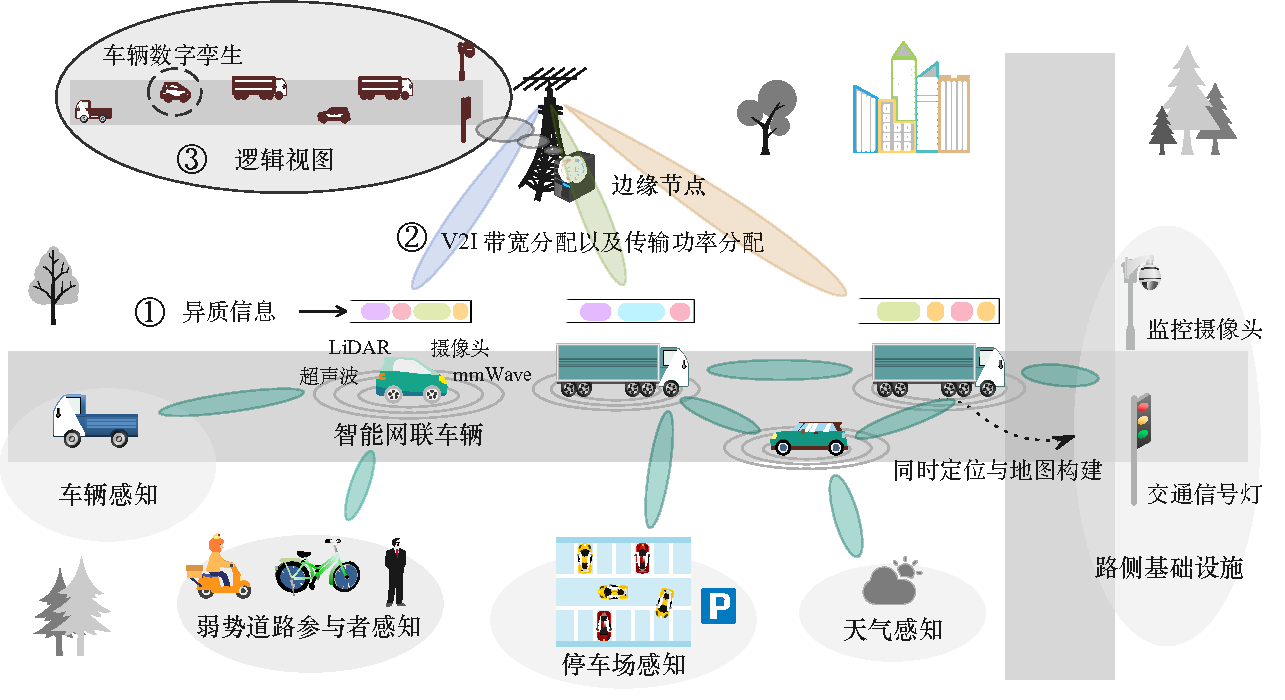
\includegraphics[width=1\columnwidth]{Fig5-1-architerture.pdf}
  \bicaption{车载信息物理融合架构}{Vehicular cyber-physical architecture}
  \label{fig 5-1}
\end{figure} 

本章节介绍了车载信息物理融合架构,如图\ref{fig 5-1}所示。
在本架构中,配备各种车载感知器,如超声波感知器、LiDAR、光学相机和毫米波雷达的车辆可以对环境进行感知。
并通过车辆间协同感知,以获得包括其他车辆、道路使用者、停车场和路边基础设施的状态在内的异质信息。
这些信息可用于在边缘节点中建立数字孪生模型,并进一步用于逻辑视图的构建,以实现各种ITS应用,如同步定位和测绘(Simultaneous Localization and Mapping,简称 SLAM)和自主交叉口控制系统。
其中,逻辑视图需要融合车辆网络中物理实体的不同信息模式,以更好地反映实时物理车辆环境,从而提高ITS的性能。
然而,构建高质量的逻辑视图可能需要更高的感知频率、更多的信息上传量和更高的能量消耗。

本系统的工作流程如下。
首先,车辆感知并排队上传不同物理实体的实时状态。
接着,边缘节点会将V2I带宽分配给车辆,并在此基础上让每辆车确定传输功率。
物理实体的数字孪生是基于从车辆收到的异质信息进行融合建立的。
需要注意的是,在这样的系统中,异质信息是由车辆以不同的感知频率感应到的,因此上传时的新鲜度会不同。
虽然增加感知频率可以提高新鲜度,但会增加排队延迟和能源消耗。
此外,多个车辆可能感知到特定物理实体的信息,若由所有车辆上传,则可能会浪费通信资源。
因此,为了提高资源利用率,需要有效而经济地分配通信资源。
在此基础上,为了最大化面向车载边缘计算的数字孪生的VCPS质量并最小化VCPS 开销,必须量化衡量边缘节点构建的数字孪生的质量和开销,并设计高效经济的协同感知和上传的调度机制。

\section{系统模型}\label{section 5-3}
\subsection{基本符号}
本系统离散时间片的集合用$\mathbf{T}=\left\{1,\ldots,t,\ldots, T \right\}$表示,其中$T$是时间片的数量。
让$\mathbf{D}$表示异质信息集合,每个信息$d \in \mathbf{D}$的特征是一个三元组$d=\left(\operatorname{type}_d, u_d, \left|d\right| \right)$,其中$\operatorname{type}_d$、$u_d$和$\left|d\right|$分别是信息类型、更新间隔和数据大小。
用$\mathbf{V}$表示车辆的集合,每个车辆$v\in \mathbf{V}$的特征是一个三元组$v=\left (l_v^t, \mathbf{D}_v, \pi_v \right )$,其中$l_v^t$, $\mathbf{D}_v$和$\pi_v$分别是位置、感知的信息集和传输功率。
对于$d \in \mathbf{D}_v$,车辆$v$的感应开销(即能耗)用$\phi_{d, v}$表示。
让$\mathbf{E}$表示边缘节点的集合。
每个边缘节点$e \in \mathbf{E}$的特征是$e=\left (l_e, g_e, b_e \right)$,其中$l_{e}$、$r_{e}$和$b_{e}$分别为位置、通信范围和带宽。
车辆$v$与边缘节点$e$之间的距离用$\operatorname{dis}_{v, e}^t \triangleq \operatorname{distance} \left (l_v^t, l_e \right ), \forall v \in \mathbf{V}, \forall e \in \mathbf{E}, \forall t \in \mathbf{T}$表示。
在$t$时间内处于边缘节点$e$的无线电覆盖范围内的车辆集合表示为$\mathbf{V}_e^t=\left \{s \vert \operatorname{dis}_{v, e}^t \leq g_e, \forall v \in \mathbf{V} \right \}, \mathbf{V}_e^t \subseteq \mathbf{V}$。

感知决策指示器表明信息$d$在时间$t$是否被车辆$v$感应到,其用以下方式表示
\begin{equation}
	c_{d, v}^t \in \{0, 1\}, \forall d \in \mathbf{D}_{v}, \forall v \in \mathbf{V}, \forall t \in \mathbf{T}
	\label{equ 5-1} 
\end{equation}
那么,车辆$v$在时间$t$感应到的信息集合表示为 $\mathbf{D}_v^t = \{ d | c_{d, v}^{t} = 1, \forall d \in \mathbf{D}_v \}, \mathbf{D}_v^t \subseteq \mathbf{D}_v$。
对于任何信息$d \in \mathbf{D}_v^t$来说,信息类型都是不同的, 即$\operatorname{type}_{d^*} \neq \operatorname{type}_{d}, \forall d^* \in \mathbf{D}_v^t \setminus \left\{ d\right \}, \forall d \in \mathbf{D}_v^t$。
车辆$v$在时间$t$的信息$d$的感知频率用$\lambda_{d, v}^t$表示,它应该满足车辆$v$的感应能力要求。
\begin{equation}
	\lambda_{d, v}^{t} \in [\lambda_{d, v}^{\min} , \lambda_{d, v}^{\max} ], \ \forall d \in \mathbf{D}_v^t, \forall v \in \mathbf{V}, \forall t \in \mathbf{T}
\end{equation}
其中$\lambda_{d, v}^{\min}$和$\lambda_{d, v}^{\max}$分别是车辆$v$中信息${d}$的最小和最大感知频率。
车辆$v$中的信息$d$在时间$t$的上传优先级用$p_{d, v}^t$表示,其需满足各不相同,即
\begin{equation}
	{p}_{d^*, v}^t \neq {p}_{d, v}^t, \forall d^* \in \mathbf{D}_v^t \setminus \left\{ d\right \}, \forall d \in \mathbf{D}_v^t, \forall v \in \mathbf{V}, \forall t \in \mathbf{T}
\end{equation}
其中${p}_{d^*, v}^t$是信息$d^* \in \mathbf{D}_v^t$中的上传优先级。
车辆$v$在时间$t$的传输功率用$\pi_{v}^t$表示,它不能超过车辆$v$的功率容量。
\begin{equation}
	\pi_v^t \in \left[ 0 , \pi_v \right ], \forall v \in \mathbf{V}, \forall t \in \mathbf{T}
\end{equation}
边缘节点$e$在$t$时间为车辆$v$分配的V2I带宽用$b_{v, e}^t$表示,且 
\begin{equation}
	b_{v, e}^t \in \left [0, b_e \right], \forall v \in \mathbf{V}_e^{t}, \forall e \in \mathbf{E}, \forall t \in \mathbf{T}
	\label{equ 5-5} 
\end{equation}
边缘节点$e$分配的V2I总带宽不能超过其容量$b_e$,即${\sum_{\forall v \in \mathbf{V}_e^{t}} b_{v, e}^t} \leq b_e, \forall t \in \mathbf{T}$。

用$j^{\prime}$表示物理实体,如车辆、行人和路边的基础设施,在VEC中表示物理实体的集合为 $\mathbf{J}^{\prime}$。
$\mathbf{D}_{j^{\prime}}$是与实体$j^{\prime}$相关的信息集合,可以用$\mathbf{D}_{j^{\prime}}=\left\{d \mid y_{d,j^{\prime}} = 1, \forall d \in \mathbf{D} \right\}$, $\forall j^{\prime} \in \mathbf{J}^{\prime}$表示, 其中$y_{d, j^{\prime}}$是一个二进制数,表示信息$d$是否由实体$j^{\prime}$关联。
$\mathbf{D}_{j^{\prime}}$的大小用$|\mathbf{D}_{j^{\prime}}|$表示。
每个实体可能需要多个信息,即$|\mathbf{D}_{j^{\prime}}| = \sum_{\forall d \in \mathbf{D}}y_{d, j^{\prime}} \geq 1, \forall j^{\prime} \in \mathbf{J}^{\prime}$。
对于每个实体$j^{\prime} \in \mathbf{J}^{\prime}$,可能有一个数字孪生$j$在边缘节点中建模。
用$\mathbf{J}$表示数字孪生的集合,用$\mathbf{J}_e^{t}$表示时间为$t$时在边缘节点$e$中建模的数字孪生集合。
因此,边缘节点$e$收到的、数字孪生$j$需要的信息集合可以用$\mathbf{D}_{j, e}^t=\bigcup_{\forall v \in \mathbf{V}}\left(\mathbf{D}_{j^{\prime}} \cap \mathbf{D}_{v, e}^t\right), \forall j \in \mathbf{J}_e^{t}, \forall e \in \mathbf{E}$表示,且 $| \mathbf{D}_{j, e}^t |$是边缘节点$e$收到的、数字孪生$j$需要的信息数量,其计算公式为$| \mathbf{D}_{j, e}^t | =  \sum_{\forall v \in \mathbf{V}} \sum_{\forall d \in \mathbf{D}_v} c_{d, v}^t  y_{d, j^{\prime}}$。

\subsection{分布式感知模型}
车辆分布式感知是基于多类M/G/1优先级队列\cite{moltafet2020age}进行建模。
假设具有$\operatorname{type}_d$的信息的上传时间$\operatorname{\hat{g}}_{d, v, e}^t$遵循均值$\alpha_{d, v}^t$和方差$\beta_{d, v}^t$的一类一般分布。
那么,车辆$v$中的上传负载$\rho_{v}^{t}$由$ \rho_{v}^{t}=\sum_{\forall d \subseteq \mathbf{D}_v^t} \lambda_{d, v}^{t} \alpha_{d, v}^t$表示。
根据多类M/G/1优先级队列的原理,需要$\rho_{v}^{t} < 1$才能达到队列的稳定状态。
信息$d$在时间$t$之前的到达时间用$\operatorname{a}_{d, v}^t$表示,其计算公式为
\begin{equation}
    \operatorname{a}_{d, v}^t = { {1}/{\lambda_{d, v}^{t}} \left \lfloor t \lambda_{d, v}^t \right \rfloor} 
\end{equation}
在时间$t$之前,由$\operatorname{u}_{d, v}^t$表示的信息$d$的更新时间是通过以下方式计算的
\begin{equation}
    \operatorname{u}_{d, v}^t = \left \lfloor  {\operatorname{a}_{d, v}^t}/{u_d} \right \rfloor  u_d
\end{equation}
其中$u_d$是信息$d$的更新间隔时间。


在$t$时间,车辆$v$中比$d$有更高上传优先权的元素集合,用$\mathbf{D}_{d, v}^t = \{ d^* \mid p_{d^*, v}^{t} > p_{d, v}^{t} , \forall d^* \in \mathbf{D}_v^t \}$,其中$p_{d^*, v}^{t}$是信息$d^* \in \mathbf{D}_v^t$的上传优先级。
因此,信息$d$前面的上传负载(即$v$在时间$t$时要在$d$之前上传的元素数量)通过以下方式计算得出 
\begin{equation}
	\rho_{d, v}^{t}=\sum_{\forall d^* \in \mathbf{D}_{d, v}^t} \lambda_{d^*, v}^t \alpha_{d^*, v}^t
\end{equation}
其中$\lambda_{d^*, v}^t$和$\alpha_{d^*, v}^t$分别为$t$时间内车辆$v$中信息$d^*$的感知频率和平均传输时间。
根据Pollaczek-Khintchine公式\cite{takine2001queue},车辆$v$中信息$d$的排队时间计算如下 
\begin{equation}
    \operatorname{q}_{d, v}^t= \frac{1} {1 - \rho_{d, v}^{t}} 
        \left[ \alpha_{d, v}^t + \frac{ \lambda_{d, v}^{t} \beta_{d, v}^t + \sum\limits_{\forall d^* \in \mathbf{D}_{d, v}^t} \lambda_{d^*, v}^t \beta_{d^*, v}^t }{2\left(1-\rho_{d, v}^{t} - \lambda_{d, v}^{t} \alpha_{d, v}^t\right)}\right] 
        - \alpha_{d, v}^t
\end{equation}

\subsection{V2I协同上传模型}
V2I的上传是基于信道衰减分布和信噪比阈值来建模的。
车辆$v$和边缘节点$e$之间的V2I通信在时间$t$的信噪比通过以下方式计算\cite{sadek2009distributed}
\begin{equation}
    \operatorname{SNR}_{v, e}^{t}=\frac{1}{N_{0}} \left|h_{v, e}\right|^{2} \tau {\operatorname{dis}_{v, e}^{t}}^{-\varphi} {\pi}_v^t
\end{equation}
其中$N_{0}$为加性白高斯噪声;$h_{v, e}$为信道衰减增益;$\tau$为常数,取决于天线设计,$\varphi$为路径损耗指数。
假设$\left|h_{v, e}\right|^{2}$遵循均值$\mu_{v, e}$和方差$\sigma_{v, e}$的一类分布,其表示方法为
\begin{equation}
    \tilde{p}=\left\{\mathbb{P}: \mathbb{E}_{\mathbb{P}}\left[\left|h_{v, e}\right|^{2}\right]=\mu_{v, e}, \mathbb{E}_{\mathbb{P}}\left[\left|h_{v, e}\right|^{2}-\mu_{v, e}\right]^{2}=\sigma_{v, e}\right\}
\end{equation}
传输可靠性是由成功传输概率超过可靠性阈值的可能性来衡量的。
\begin{equation}
    \inf_{\mathbb{P} \in \tilde{p}} \operatorname{Pr}_{[\mathbb{P}]}\left(\operatorname{SNR}_{v, e}^{t} \geq \operatorname{SNR}_{v, e}^{\operatorname{tgt}}\right) \geq \delta
\end{equation}
\noindent 其中$\operatorname{SNR}_{v, e}^{\operatorname{tgt}}$和$\delta$分别为目标SNR阈值和可靠性阈值。
由车辆$v$上传并由边缘节点$e$接收的信息集合用$\mathbf{D}_{v, e}^{t} = \bigcup_{\forall v \in \mathbf{V}_{e}^{t}} \mathbf{D}_{v}^{t}$表示。

根据香农理论,车辆$v$和边缘节点$e$之间在$t$时间的V2I通信的传输率用$\operatorname{z}_{v, e}^t$表示,计算结果为
\begin{equation}
    \operatorname{z}_{v, e}^t=b_{v}^{t} \log _{2}\left(1+\mathrm{SNR}_{v, e}^{t}\right)
\end{equation}
假设车辆$v$被安排在时间$t$上传$d$,并且$d$将在一定的排队时间$\mathrm{\bar{q}}_{d, v}^t$后被传输。
然后,本章把车辆$v$开始传输$d$的时刻表示为$\mathrm{t}_{d, v}^t=t+\mathrm{q}_{d, v}^t$。
从$\mathrm{t}_{d, v}^t$到$\mathrm{t}_{d, v}^t + f$之间传输的数据量可由 $\int_{\mathrm{t}_{d, v}^t}^{\mathrm{t}_{d, v}^t+f} \mathrm{z}_{v, e}^t \mathrm{~d} t$ bits 得到,其中$f \in \mathbb{R}^{+}$和$\mathrm{z}_{j, e}^t$是时间$t$的传输速率。
如果在整个传输过程中可以传输的数据量大于信息$d$的大小,那么上传就会完成。
因此,从车辆$v$到边缘节点$e$传输信息$d$的时间,用$\operatorname{g}_{d, v, e}^t$表示,计算如下 
\begin{equation}
    \operatorname{g}_{d, v, e}^t=\inf _{j \in \mathbb{R}^+} \left \{ \int_{\operatorname{k}_{d, v}^t}^{\operatorname{k}_{d, v}^t + j} {\operatorname{z}_{v, e}^t} \operatorname{d}t \geq \left|d\right| \right \} 
\end{equation}
\noindent 其中$\operatorname{t}_{d, v}^t = t +\operatorname{q}_{d, v}^t$是车辆$v$开始传输信息$d$的时刻。

\section{问题定义}\label{section 5-4}

\subsection{VCPS质量}
首先,由于数字孪生是基于连续上传和时间变化的信息建模的,本章对信息的及时性$d$的定义如下。
\begin{definition}[\textbf{信息 $d$的时效性}]
信息$d$在车辆$v$中的实效性$\theta_{d, v} \in \mathbb{Q}^{+}$被定义为更新和接收信息$d$之间的时间。
\begin{equation}
    \theta_{d, v} = \operatorname{a}_{d, v}^t + \operatorname{q}_{d, v}^t + \operatorname{g}_{d, v, e}^t-\operatorname{u}_{d, v}^{t}, \forall d \in \mathbf{D}_v^t,\forall v \in \mathbf{V}
\end{equation}
\end{definition}
\begin{definition}[\textbf{数字孪生$j$ 的时效性}]
数字孪生$j$的及时性 $\Theta_{j} \in \mathbb{Q}^{+}$被定义为与物理实体$j^{\prime}$相关的信息的最大及时性之和。
	\begin{equation}
    	\Theta_{j} = \sum_{\forall v\in \mathbf{V}_{e}^{t}} \max_{\forall d \in \mathbf{D}_{j^{\prime}} \cap \mathbf{D}_v^t}\theta_{d, v}, \forall j \in \mathbf{J}_{e}^{t}, \forall e \in \mathbf{E}
    	\label{equ 5-16}
	\end{equation}
\end{definition}

其次,由于不同类型的信息有不同的感知频率和上传优先级,本章定义数字孪生的一致性来衡量与同一物理实体相关的信息的一致性。
\begin{definition}[\textbf{数字孪生$j$的一致性}]
数字孪生$j$的一致性$\Psi_{j} \in \mathbb{Q}^{+}$被定义为信息更新时间差的最大值。
\begin{equation}
    \Psi_{j}=\max_{\forall d \in \mathbf{D}_{j, e}^{t}, \forall v \in \mathbf{V}_{e}^{t}} {\operatorname{u}_{d, v}^t} - \min_{\forall d \in \mathbf{D}_{j, e}^{t}, \forall v \in \mathbf{V}_{e}^{t}} {\operatorname{u}_{d, v}^t} , \forall j \in \mathbf{J}_{e}^{t}, \forall e \in \mathbf{E}
\end{equation}
\end{definition}

最后,本章给出了数字孪生的质量的正式定义,其综合了数字孪生的及时性和一致性。
\begin{definition}[\textbf{数字孪生质量, QDT}]
数字孪生$\operatorname{QDT}_{j} \in (0, 1)$的质量被定义为数字孪生$j$的归一化及时性和归一化一致性的加权平均和。
	\begin{equation}
	    \operatorname{QDT}_{j} = w_1 (1 -\hat{\Theta_{j}}) + w_2 (1 - \hat{\Psi_{j}}), \forall j \in \mathbf{J}_{e}^t, \forall e \in \mathbf{E}
	\end{equation}
\end{definition}
\noindent 其中$\hat{\Theta_{j}} \in (0, 1)$和$\hat{\Psi_{j}} \in (0, 1)$分别表示归一化的时效性和归一化的一致性,这可以通过最小-最大归一化对时效性和一致性的范围进行重新调整至$(0, 1)$来获得。
$\hat{\Theta_{j}}$和$\hat{\Psi_{j}}$的加权系数分别用$w_1$和$w_2$表示,可以根据ITS应用的不同要求进行相应的调整,本章有$w_1+w_2=1$。
进一步,基于数字孪生质量定义车载信息物理融合系统的质量,具体如下
\begin{definition}[\textbf{VCPS质量}]
VCPS质量$\mathscr{Q} \in (0, 1)$被定义为在调度期间$\mathbf{T}$的边缘节点中建模的每个数字孪生的QDT的平均值。
	\begin{equation}
		\mathscr{Q}=\frac{\sum_{\forall t \in \mathbf{T}} \sum_{\forall e \in \mathbf{E}} \sum_{\forall j \in \mathbf{J}_e^t} \operatorname{QDT}_{j}}{\sum_{\forall t \in \mathbf{T}} \sum_{\forall e \in \mathbf{E}} |\mathbf{J}_e^t| }
	\end{equation}
\end{definition}

\subsection{VCPS开销}

首先,由于同一物理实体的状态可能被多个车辆同时感应到,本章对信息的冗余度$d$定义如下。
\begin{definition}[\textbf{信息$d$的冗余度}]
信息$d$的冗余度$\xi_d \in \mathbb{N}$被定义为车辆感应到的具有$\operatorname{type}_d$的额外信息数量。
\begin{equation}
    \xi_d= \left | \mathbf{D}_{d, j, e} \right| - 1, \forall d \in \mathbf{D}_j, \forall j \in \mathbf{J}_{e}^{t}, \forall e \in \mathbf{E}
\end{equation}
\noindent 其中$\mathbf{D}_{d, j, e}$是边缘节点$e$收到的、数字孪生$j$需要的具有$\operatorname{type}_d$的信息集合。它由$\mathbf{D}_{d, j, e}=\left\{ d^* \vert \operatorname{type}_{d^*} = \operatorname{type}_{d}, \forall d^* \in \mathbf{D}_{j, e}^t \right \}$表示。

\end{definition}
\begin{definition}[\textbf{数字孪生 $j$的冗余度}]
数字孪生$j$的冗余度$\Xi_j \in \mathbb{N}$被定义为数字孪生$j$中的总冗余度。
	\begin{equation}
       \Xi_j =  \sum_{\forall d \in \mathbf{D}_{j^{\prime}}} \xi_d, \forall j \in \mathbf{J}_{e}^{t}, \forall e \in \mathbf{E}
       \label{equ 5-20}
    \end{equation}
\end{definition}

其次,信息感知和传输需要消耗车辆的能量,本章定义数字孪生$j$的感知开销和传输开销如下。
\begin{definition}[\textbf{数字孪生 $j$ 的感知开销}]
数字孪生$j$的感知开销$\Phi_{j} \in \mathbb{Q}^{+}$被定义为数字孪生$j$所需信息的总感应开销。
	\begin{equation}
        \Phi_{j} = \sum_{\forall v \in \mathbf{V}_{e}^{t}} \sum_{\forall d \in \mathbf{D}_{j^{\prime}} \cap \mathbf{D}_v^t}{\phi_{d, v}}, \forall j \in \mathbf{J}_{e}^t, \forall e \in \mathbf{E}
        \label{equ 5-21}
    \end{equation}
    其中$\phi_{d, v}$是信息$d$在车辆$v$中的感应开销。
\end{definition}
\begin{definition}[\textbf{信息$d$的传输开销}]
信息$d$在车辆$v$中的传输开销${\omega}_{d, v} \in \mathbb{Q}^{+}$被定义为信息上传时消耗的传输功率。
\begin{equation}
    {\omega}_{d, v}= \pi_v^t \operatorname{g}_{d, v, e}^t, \forall d \in \mathbf{D}_v^t
\end{equation}
其中$\pi_v^t$和$\operatorname{g}_{d, v, e}^t$分别为传输功率和传输时间。
\end{definition}
\begin{definition}[\textbf{数字孪生$j$ 的传输开销}]
数字孪生$j$的传输开销$\Omega_{j} \in \mathbb{Q}^{+}$被定义为数字孪生$j$所需的信息总传输开销。
	\begin{equation}
        \Omega_{j} = \sum_{\forall v \in \mathbf{V}_{e}^{t}} \sum_{\forall d \in \mathbf{D}_{j^{\prime}} \cap \mathbf{D}_v^t} {\omega}_{d, v}, \forall j \in \mathbf{J}_{e}^t, \forall e \in \mathbf{E}
       	\label{equ 5-23}
    \end{equation}
\end{definition}

最后,本章给出了数字孪生开销的正式定义,综合了冗余度、感知开销和传输开销。
\begin{definition}[\textbf{数字孪生开销, CDT}]
数字孪生的开销$\operatorname{CDT}_{j} \in (0, 1)$被定义为数字孪生$j$的正常化冗余、正常化感知开销和正常化传输开销的加权平均和。
	\begin{equation}
	    \operatorname{CDT}_{j} = w_3  \hat{\Xi_{j}} +  w_4 \hat{\Phi_{j}} + w_5 \hat{\Omega_{j}}, \forall j \in \mathbf{J}_{e}^t, \forall e \in \mathbf{E}
	\end{equation}
\end{definition}
\noindent 其中 $\hat{\Xi_{j}}\in (0, 1)$、$\hat{\Phi_{j}} \in (0, 1)$和$\hat{\Omega_{j}} \in (0, 1)$ 分别表示数字孪生$j$的归一化冗余度、归一化感知开销和归一化传输开销。
$\hat{\Xi_{j}}$、$\hat{\Phi_{j}}$和$\hat{\Omega_{j}}$ 的加权系数分别表示为 $w_3$、$w_4$和 $w_5$。
同样地,$w_3+w_4+w_5=1$。
进一步,VCPS开销定义如下。
\begin{definition}[\textbf{VCPS 开销}]
VCPS 开销$\mathscr{C} \in (0, 1)$被定义为$\mathbf{T}$调度期间边缘节点中每个数字孪生模型的CDT的平均值。
	\begin{equation}
		\mathscr{C}=\frac{\sum_{\forall t \in \mathbf{T}} \sum_{\forall e \in \mathbf{E}} \sum_{\forall j \in \mathbf{J}_e^t}  \operatorname{CDT}_{j}}{\sum_{\forall t \in \mathbf{T}} \sum_{\forall e \in \mathbf{E}} |\mathbf{J}_e^t| }
	\end{equation}
\end{definition}

\subsection{双目标问题}
给定一个解决方案$( \mathbf{C}, \bf\Lambda, \mathbf{P}, \bf\Pi, \mathbf{B} )$,其中$\mathbf{C}$表示确定的感应信息,$\bf\Lambda$表示确定的感知频率。$\mathbf{P}$表示确定的上传优先级,$\bf\Pi$表示确定的传输功率,$\mathbf{B}$表示确定的V2I带宽分配。
\begin{numcases}
	\mathbf{C} = \left \{ c_{d, v}^t \vert \forall d \in D_{v}, \forall v \in S, \forall t \in T \right  \} \notag \\
	\bf\Lambda = \left \{ \lambda_{d, v}^{t} \vert \forall d \in D_v^t  , \forall v \in S, \forall t \in T \right \} \notag \\ 
	\mathbf{P} = \left \{ p_{d, v}^{t} \vert \forall d \in D_v^t  , \forall v \in S, \forall t \in T\right \}  \notag \\
	\bf\Pi = \left \{ \pi_v^t \vert \forall v \in S, \forall t \in T \right \} \notag \\
	\mathbf{B} = \left \{ b_v^t \vert \forall v \in S, \forall t \in T\right \}
\end{numcases}
其中$c_{d, v}^t$、$\lambda_{d, v}^{t}$和$p_{d, v}^{t}$分别为$t$时间内车辆$v$的信息$d$的感应决策、感知频率和上传优先权,$\pi_v^t$和$b_v^t$分别为$t$时间内车辆$v$的传输功率和V2I带宽。
本章提出了一个双目标问题,旨在同时实现VCPS质量的最大化和VCPS 开销的最小化,该问题表示为
\begin{align}
	\mathcal{P}5.1: & \max_{\mathbf{C}, \bf\Lambda, \mathbf{P}, \bf\Pi, \mathbf{B}} \mathscr{Q}, \min_{\mathbf{C}, \bf\Lambda, \mathbf{P}, \bf\Pi, \mathbf{B}} \mathscr{C} \notag \\
	\text { s.t. }
	& (\ref{equ 5-1}) \sim (\ref{equ 5-5}) \notag \\
    &\mathcal{C}5.1: \sum_{\forall d \subseteq \mathbf{D}_v^t} \lambda_{d, v}^{t} \mu_d<1,\ \forall v \in \mathbf{V}, \forall t \in \mathbf{T} \notag \\
    &\mathcal{C}5.2: \inf_{\mathbb{P} \in \tilde{p}} \operatorname{Pr}_{[\mathbb{P}]}\left(\operatorname{SNR}_{v, e}^{t} \geq \operatorname{SNR}_{v, e}^{\operatorname{tgt}}\right) \geq \delta, \forall v \in \mathbf{V}, \forall t \in \mathbf{T} \notag \\
    &\mathcal{C}5.3: {\sum_{\forall v \in \mathbf{V}_e^{t}}b_v^t} \leq b_e, \forall t \in \mathbf{T}
\end{align}
其中$\mathcal{C}5.1$保证队列稳定状态,$\mathcal{C}5.2$保证传输可靠性。
$\mathcal{C}5.3$要求边缘节点$e$分配的V2I带宽之和不能超过其容量$b_e$。
根据CDT的定义,本章将数字孪生的利润定义如下。
\begin{definition}[\textbf{数字孪生利润, PDT}]
数字孪生的利润$\operatorname{PDT}_{j} \in (0, 1)$被定义为数字孪生$j$的CDT的补充。
	\begin{equation}
		\mathscr{P}= 1 - \operatorname{CDT}_{j}
	\end{equation}
\end{definition}
\noindent 然后,本章将VCPS 利润定义如下。
\begin{definition}[\textbf{VCPS 利润}]
VCPS 利润$\mathscr{P} \in (0, 1)$被定义为在调度期$\mathbf{T}$期间,边缘节点中每个数字孪生模型的PDT的平均值。
	\begin{equation}
		\mathscr{P}= \frac{\sum_{\forall t \in \mathbf{T}} \sum_{\forall e \in \mathbf{E}} \sum_{\forall j \in \mathbf{J}_e^t}   \operatorname{PDT}_{j} }{\sum_{\forall t \in \mathbf{T}} \sum_{\forall e \in \mathbf{E}} |\mathbf{J}_e^t| }
	\end{equation}
\end{definition}
\noindent 因此,$\mathcal{P}5.1$问题可以改写为如下。
\begin{align}
	\mathcal{P}5.2: & \max_{( \mathbf{C}, \bf\Lambda, \mathbf{P}, \bf\Pi, \mathbf{B} )} \left (\mathscr{Q}, \mathscr{P} \right ) \notag \\
		\text { s.t. }
	&(\ref{equ 5-1}) \sim (\ref{equ 5-5}), \mathcal{C}5.1 \sim \mathcal{C}5.3
\end{align}

\section{算法设计}\label{section 5-5}

\begin{figure}[h]
\centering
  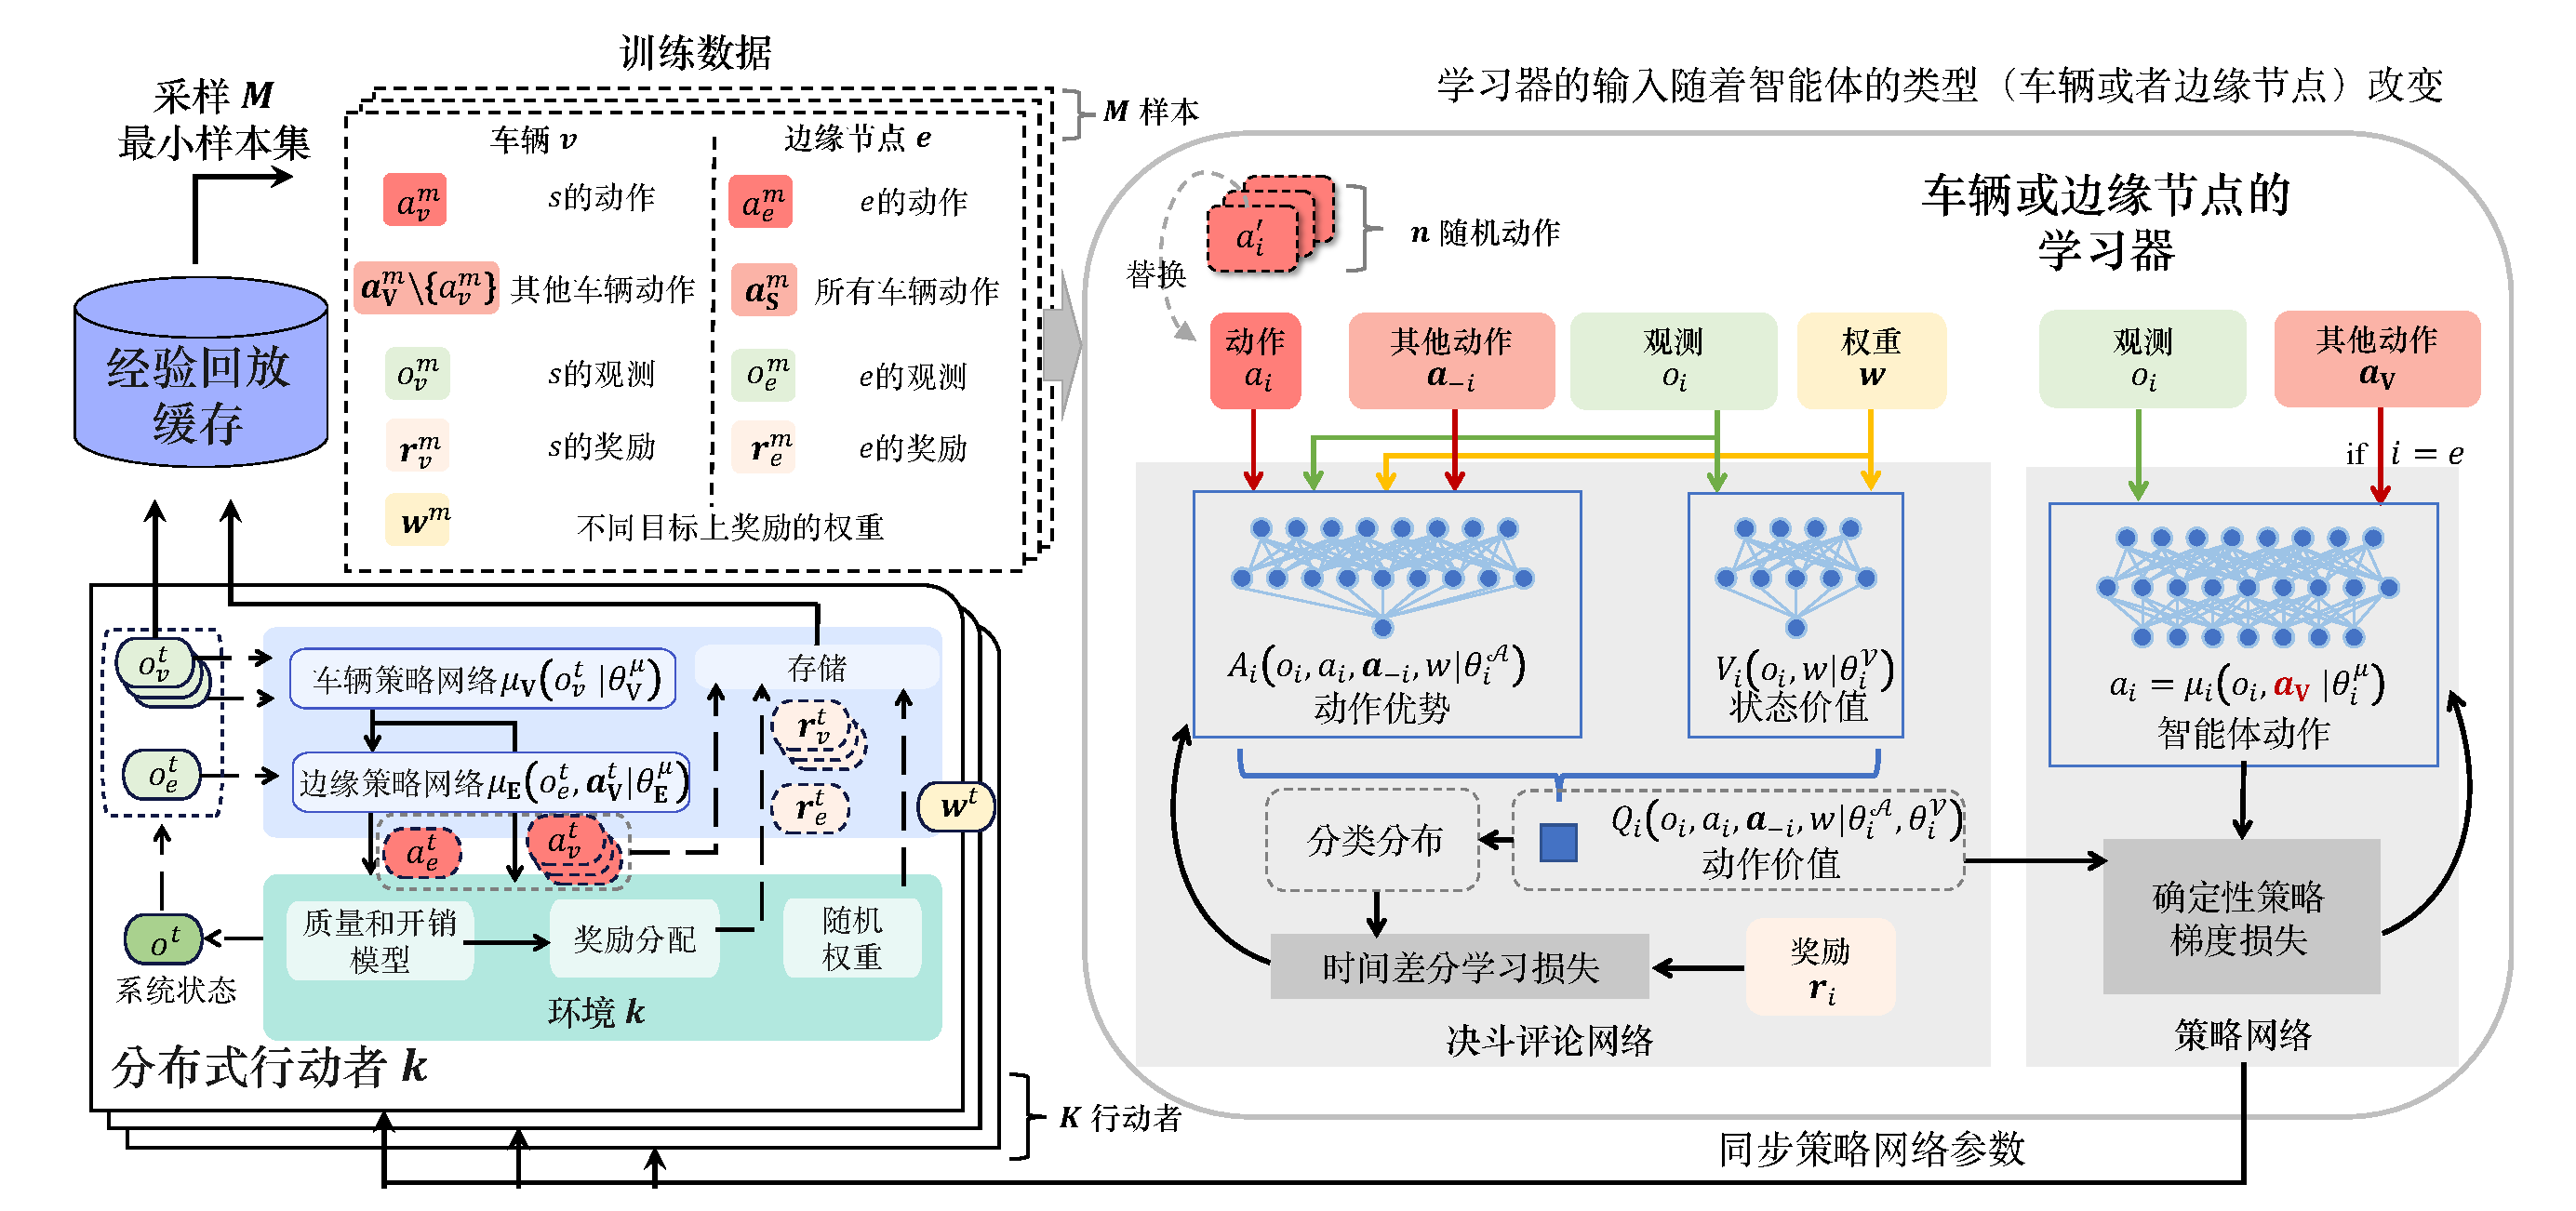
\includegraphics[width=1\columnwidth]{Fig5-2-solution-model.pdf}
  \bicaption{多智能体多目标深度强化学习算法模型}{Multi-agent multi-objective deep reinforcement learning model}
  \label{fig 5-2}
\end{figure}

在本章节中,提出了一个基于多智能体多目标深度强化学习的解决方案。
该解决方案的一般模型如图\ref{fig 5-2}所示,它由$K$分布式智能体、学习器和经验回放缓存组成。
具体来说,学习器由四个神经网络组成,即一个本地策略网络、一个本地评论家网络、一个目标策略网络和一个目标评论家网络,其中车辆的参数表示为 $\theta_{\mathbf{V}}^{\mu}$、$\theta_{\mathbf{V}}^{Q}$、 $\theta_{\mathbf{V}}^{\mu^{\prime}}$和$\theta_{\mathbf{V}}^{Q^{\prime}}$。
同样地,四个网络的边缘节点的参数表示为 $\theta_{\mathbf{E}}^{\mu}$、$\theta_{\mathbf{E}}^{Q}$、$\theta_{\mathbf{E}}^{\mu^{\prime}}$和$\theta_{\mathbf{E}}^{Q^{\prime}}$。
本地策略和本地评论家网络的参数是随机初始化的。
目标策略和目标评论家网络的参数被初始化为相应的本地网络。
启动$K$分布式行为体,与环境进行交互,并执行重放经验存储。
每个智能体由一个本地车辆策略网络和一个本地边缘策略网络组成,分别用$\theta_{\mathbf{V}, k}^{\mu}$和$\theta_{\mathbf{E}, k}^{\mu}$表示,它们是由学习器的本地策略网络复制而来的。
最大尺寸为$\mathcal{B}$的经验回放缓存被初始化以存储重放经验。

\subsection{多智能体分布式策略执行}

在MAMO中,车辆和边缘节点通过本地策略网络以分布式的方式决定他们的行动。
车辆$v$在时间$t$上对系统状态的局部观测表示为 
	\begin{equation}
		\boldsymbol{o}_{v}^{t}=\left\{t, v, l_{v}^t, \mathbf{D}_{v}, \Phi_{v}, \mathbf{D}_{e}^{t}, \mathbf{D}_{\mathbf{J}_e^t}, \boldsymbol{w}^{t}\right\}
	\end{equation} 
\noindent 其中$t$为时隙指数。
$v$是车辆索引;$l_{v}^t$是车辆$v$的位置。
$\mathbf{D}_{v}$表示车辆$v$可以感知的信息集合。
$\Phi_{v}$代表$\mathbf{D}_{v}$中信息的感应开销。
$\mathbf{D}_{e}^{t}$ 代表$e$在时间$t$的边缘节点的缓存信息集。
$\mathbf{D}_{\mathbf{J}_e^t}$ 代表在时间$t$的边缘节点$e$中建模的数字孪生所需的信息集,且 $\boldsymbol{w}^{t}$ 代表每个目标的权重向量,它在每次迭代中随机生成。
具体来说,$\boldsymbol{w}^{t} = \begin{bmatrix}  w^{(1), t}  &  w^{(2), t} \end{bmatrix}$,其中$w^{(1), t} \in (0, 1)$和$w^{(2), t} \in (0, 1)$分别是VCPS质量和VCPS 利润的权重,本章有$\sum_{\forall j \in \{1, 2\}} w^{(j), t} = 1$。
另一方面,边缘节点$e$在时间$t$上对系统状态的局部观测表示为
\begin{equation}
	\boldsymbol{o}_{e}^{t}=\left\{t, e, \operatorname{\mathbf{Dis}}_{\mathbf{V}, e}^{t}, \mathbf{D}_{1}, \ldots, \mathbf{D}_{v}, \ldots, \mathbf{D}_{v}, \mathbf{D}_{e}^{t}, \mathbf{D}_{\mathbf{J}_e^t}, \boldsymbol{w}^{t} \right\}
\end{equation}
\noindent 其中$e$是边缘节点索引,$\operatorname{\mathbf{Dis}}_{\mathbf{V}, e}^{t}$代表车辆与边缘节点$e$之间的距离集合。
因此,系统在时间$t$的状态可以表示为$\boldsymbol{o}^{t}=\boldsymbol{o}_{e}^{t} \cup \boldsymbol{o}_{1}^{t} \cup \ldots \cup \boldsymbol{o}_{v}^{t} \cup \ldots \cup \boldsymbol{o}_{v}^{t}$。

车辆$v$的动作表示为 
\begin{equation}
	\boldsymbol{a}_{v}^{t} = \{ \mathbf{C}_v^t,  \{ \lambda_{d, v}^{t}, p_{d, v}^{t} \mid \forall d \in \mathbf{D}_{v}^t \} , \pi_v^t   \}
\end{equation}
其中,$\mathbf{C}_v^t$是感知决策;$\lambda_{d, v}^{t}$和$p_{d, v}^{t}$分别是信息$d$的感知频率和上传优先级,$\pi_v^t$是车辆$v$在时间$t$的传输功率。
车辆动作是由本地车辆策略网络根据其对系统状态的本地观测而产生的。
\begin{equation}
	\boldsymbol{a}_{v}^{t}=\mu_{\mathbf{V}}\left(\boldsymbol{o}_{v}^{t} \mid \theta_{\mathbf{V}}^{\mu}\right)+\epsilon_{v} \mathcal{N}_{v}^{t}
\end{equation}
\noindent 其中,$\mathcal{N}_{v}^{t}$为探索噪音,以增加车辆动作的多样性,$\epsilon_{v}$为车辆$v$的探索常数。
车辆动作的集合被表示为 $\boldsymbol{a}_{\mathbf{V}}^{t} = \left\{\boldsymbol{a}_{v}^{t}\mid \forall v \in \mathbf{V}\right\}$。
那么,边缘节点$e$的动作表示为
\begin{equation}
	\boldsymbol{a}_{e}^{t} = \{b_{v, e}^{t} \mid \forall v \in \mathbf{V}_{e}^{t}\}
\end{equation}
其中$b_{v, e}^t$是边缘节点$e$在时间$t$为车辆$v$分配的V2I带宽。
同样,边缘节点$e$的动作可以由本地边缘策略网络根据系统状态以及车辆动作得到。
\begin{equation}
	\boldsymbol{a}_{e}^{t}=\mu_{\mathbf{E}}\left(\boldsymbol{o}_{e}^{t},  \boldsymbol{a}_{\boldsymbol{\mathbf{V}}}^{t} \mid \theta_{\mathbf{E}}^{\mu}\right)+\epsilon_{e} \mathcal{N}_{e}^{t}
\end{equation}
\noindent 其中$\mathcal{N}_{e}^{t}$和$\epsilon_{e}$分别为边缘节点$e$的探索噪声和探索常数。
此外,车辆和边缘节点的联合动作被表示为 $\boldsymbol{a}^{t}= \left\{\boldsymbol{a}_{e}^{t}, \boldsymbol{a}_{1}^{t}, \ldots, \boldsymbol{a}_{v}^{t}, \ldots, \boldsymbol{a}_{V}^{t}\right\}$。

环境通过执行联合动作获得系统奖励向量,其表示为 
	\begin{equation}
	\boldsymbol{r}^{t} = \begin{bmatrix}  r^{(1)}\left(\boldsymbol{a}_{\mathbf{V}}^{t},\boldsymbol{a}_{e}^{t} \mid \boldsymbol{o}^{t}\right)  &  r^{(2)}\left(\boldsymbol{a}_{\mathbf{V}}^{t},\boldsymbol{a}_{e}^{t} \mid \boldsymbol{o}^{t}\right) \end{bmatrix} ^{T}
	\end{equation}
	\noindent 其中 $r^{(1)}\left(\boldsymbol{a}_{\mathbf{V}}^{t},\boldsymbol{a}_{e}^{t} \mid \boldsymbol{o}^{t}\right)$ 和 $r^{(2)}\left(\boldsymbol{a}_{\mathbf{V}}^{t},\boldsymbol{a}_{e}^{t} \mid \boldsymbol{o}^{t}\right)$ 分别是两个目标(即实现的VCPS质量和VCPS 利润)的奖励,可以通过以下方式计算出来  
	\begin{numcases}{}
			r^{(1)}\left(\boldsymbol{a}_{\mathbf{V}}^{t},\boldsymbol{a}_{e}^{t} \mid \boldsymbol{o}^{t}\right)={1}/{\left|\mathbf{J}_e^t\right|} \sum_{\forall j \in \mathbf{J}_e^t}\operatorname{QDT}_{j} \notag \\
			r^{(2)}\left(\boldsymbol{a}_{\mathbf{V}}^{t},\boldsymbol{a}_{e}^{t} \mid \boldsymbol{o}^{t}\right)={1}/{\left|\mathbf{J}_e^t\right|} \sum_{\forall j \in \mathbf{J}_e^t} \operatorname{PDT}_{j} 
	\end{numcases}
因此,车辆$v$在第$j$个目标中的奖励是由基于奖励分配的差分奖励(DR) \cite{foerster2018counterfactual} 得到的,它是系统奖励和没有其行动所取得的奖励之间的差额,可以表示为 
\begin{equation}
r_{v}^{(j), t}=r^{(j)}\left(\boldsymbol{a}_{\mathbf{V}}^{t},\boldsymbol{a}_{e}^{t} \mid \boldsymbol{o}^{t}\right)-r^{(j)}\left(\boldsymbol{a}_{\mathbf{V}-s}^{t},\boldsymbol{a}_{e}^{t} \mid \boldsymbol{o}^{t}\right), \forall j \in \{1, 2\}
\end{equation}
\noindent 其中 $r^{(j)}\left(\boldsymbol{a}_{\mathbf{V}-s}^{t},\boldsymbol{a}_{e}^{t} \mid \boldsymbol{o}^{t}\right)$ 是在没有车辆$v$贡献的情况下实现的系统奖励,它可以通过设置车辆$v$的空动作集得到。
车辆$v$在时间$t$的奖励向量表示为$\boldsymbol{r}_{v}^{t} = \begin{bmatrix}  r_{v}^{(1), t}  &  r_{v}^{(2), t} \end{bmatrix} ^{T}$。
车辆的差分奖励集合表示为 $\boldsymbol{r}_{\mathbf{V}}^{t}=\{ \boldsymbol{r}_{v}^{t} \mid \forall v \in \mathbf{V}\}$.

另一方面,系统奖励通过最小-最大归一化进一步转化为边缘节点的归一化奖励。
边缘节点$e$在$t$时间的第$j$个目标中的奖励由以下方式计算 
\begin{equation}
	r_{e}^{(j), t}= \frac{r^{(j)}\left(\boldsymbol{a}_{\mathbf{V}}^{t},\boldsymbol{a}_{e}^{t} \mid \boldsymbol{o}^{t}\right) - \min \limits_{\forall {\boldsymbol{a}_{e}^{t}}^{\prime}} r^{(j)}\left(\boldsymbol{a}_{\mathbf{V}}^{t}, {\boldsymbol{a}_{e}^{t}}^{\prime} \mid \boldsymbol{o}^{t}\right)} {\max \limits_{\forall {\boldsymbol{a}_{e}^{t}}^{\prime}} r^{(j)}\left(\boldsymbol{a}_{\mathbf{V}}^{t}, {\boldsymbol{a}_{e}^{t}}^{\prime} \mid \boldsymbol{o}^{t}\right) - \min \limits_{\forall {\boldsymbol{a}_{e}^{t}}^{\prime}} r^{(j)}\left(\boldsymbol{a}_{\mathbf{V}}^{t}, {\boldsymbol{a}_{e}^{t}}^{\prime} \mid \boldsymbol{o}^{t}\right)}
\end{equation}
\noindent 其中 $\min \limits_{\forall {\boldsymbol{a}_{e}^{t}}^{\prime}} r^{(j)} (\boldsymbol{a}_{\mathbf{V}}^{t}, {\boldsymbol{a}_{e}^{t}}^{\prime} \mid \boldsymbol{o}^{t})$ 和 $\max \limits_{\forall {\boldsymbol{a}_{e}^{t}}^{\prime}} r^{(j)}(\boldsymbol{a}_{\mathbf{V}}^{t}, {\boldsymbol{a}_{e}^{t}}^{\prime} \mid \boldsymbol{o}^{t})$ 分别是在相同的系统状态$\boldsymbol{o}^{t}$下,车辆动作$\boldsymbol{a}_{\mathbf{V}}^{t}$不变时实现的系统奖励的最小值和最大值。
边缘节点$e$在时间$t$的奖励向量表示为 $\boldsymbol{r}_{e}^{t} = \begin{bmatrix}  r_{e}^{(1), t}  &  r_{e}^{(2), t} \end{bmatrix} ^{T}$。
交互经验包括系统状态$\boldsymbol{o}^{t}$,车辆动作$\boldsymbol{a}_{\mathbf{V}}^{t}$、边缘节点动作${a}_{e}^{t}$,车辆奖励$\boldsymbol{r}_{v}^{t}$、边缘节点奖励$\boldsymbol{r}_{e}^{t}$、权重$\boldsymbol{w}^{t}$,以及下一个系统状态$\boldsymbol{o}^{t+1}$,都存储到经验回放缓存$\mathcal{B}$。
这种互动将持续到学习器的训练过程结束。

\subsection{多目标策略评估}

在这一节中,本章提出了决斗评论家网络(Dueling Critic Network,简称 DCN),根据状态的价值和行动的优势来评估智能体的行动。
在DCN中有两个全连接的网络,即动作优势(Action-Advantage,简称 AA)网络和状态价值(State-Value,简称 SV)网络。
请注意,车辆和边缘节点的AA网络参数分别表示为 $\theta_{\mathbf{V}}^{\mathscr{A}}$ 和 $\theta_{\mathbf{E}}^{\mathscr{A}}$。
同样,车辆和边缘节点的SV网络的参数分别表示为 $\theta_{\mathbf{V}}^{\mathscr{V}}$ 和 $\theta_{\mathbf{E}}^{\mathscr{V}}$。
本章用以下方式表示车辆$v$中AA网络的输出标量 $A_{\mathbf{V}}\left({o}_{v}^{m},  {a}_{v}^{m}, \boldsymbol{a}_{\boldsymbol{\mathbf{V}}-v}^{m}, \boldsymbol{w}^{m} \mid \theta_{\mathbf{V}}^{\mathscr{A}} \right)$, 其中 $\boldsymbol{a}_{\boldsymbol{\mathbf{V}}-v}^{m}$ 表示其他车辆动作。
同样地,以边缘节点$e$为输入的AA网络的输出标量表示为 $A_{\mathbf{E}}\left({o}_{e}^{m},  {a}_{e}^{m}, \boldsymbol{a}_{\boldsymbol{\mathbf{V}}}^{m}, \boldsymbol{w}^{m} \mid \theta_{\mathbf{E}}^{\mathscr{A}} \right)$, 其中 $\boldsymbol{a}_{\boldsymbol{\mathbf{V}}}^{m}$ 表示所有车辆动作。
车辆$v$的SV网络的输出标量表示为 $j\left({o}_{v}^{m}, \boldsymbol{w}^{m} \mid \theta_{\mathbf{V}}^{\mathscr{V}} \right)$. 
同样地,边缘节点$e$的SV网络的输出标量表示为 $j\left({o}_{e}^{m}, \boldsymbol{w}^{m} \mid \theta_{\mathbf{E}}^{\mathscr{V}} \right)$.

智能体动作评估由三个步骤组成。
首先,AA网络通过输出基于观测、动作和权重的智能体动作的优势来估计优势函数。
第二,VS网络根据观测和权重,通过输出状态的值来估计价值函数。
第三,采用一个聚合模块,根据行动的优势和状态的价值,输出一个单一的价值来评估行动。
具体来说,在AA网络中随机生成$N$行动并替换成智能体动作,以评估随机行动的平均优势值。
本章用${a}_{v}^{m, n}$和${a}_{e}^{m, n}$分别表示车辆$v$和边缘节点$e$的第$n$随机行动。
因此,车辆$v$和边缘节点$e$的第$n$次随机行动的优势可以分别用 $A_{\mathbf{V}}\left({o}_{v}^{m},  {a}_{v}^{m, n}, \boldsymbol{a}_{\boldsymbol{\mathbf{V}}-v}^{m}, \boldsymbol{w}^{m} \mid \theta_{v}^{\mathscr{A}} \right)$ 和 $A_{\mathbf{E}}\left({o}_{e}^{m},  {a}_{e}^{m, n}, \boldsymbol{a}_{\boldsymbol{\mathbf{V}}}^{m}, \boldsymbol{w}^{m} \mid \theta_{\mathbf{E}}^{\mathscr{A}} \right)$表示。

价值函数的聚合模块是通过评估智能体动作对随机行动的平均优势来构建的。
因此,车辆$v\in\mathbf{V}$和边缘节点$e$的动作价值是通过以下方式计算的 
\begin{align}
    Q_{\mathbf{V}}\left({o}_{v}^{m}, {a}_{v}^{m}, \boldsymbol{a}_{\boldsymbol{\mathbf{V}}-v}^{m}, \boldsymbol{w}^{m} \mid \theta_{\mathbf{V}}^{Q} \right) &= V\left({o}_{v}^{m}, \boldsymbol{w}^{m} \mid \theta_{\mathbf{V}}^{\mathscr{V}} \right) + A_{\mathbf{V}}\left({o}_{v}^{m},  {a}_{v}^{m}, \boldsymbol{a}_{\boldsymbol{\mathbf{V}}-v}^{m}, \boldsymbol{w}^{m} \mid \theta_{\mathbf{V}}^{\mathscr{A}} \right) \notag \\
    &- \frac{1}{N} \sum_{\forall n} A_{\mathbf{V}}\left({o}_{v}^{m},  {a}_{v}^{m, n}, \boldsymbol{a}_{\boldsymbol{\mathbf{V}}-v}^{m}, \boldsymbol{w}^{m} \mid \theta_{\mathbf{V}}^{\mathscr{A}} \right)
\end{align}
\begin{align}
    Q_{E}\left({o}_{e}^{m},  {a}_{e}^{m}, \boldsymbol{a}_{\boldsymbol{\mathbf{V}}}^{m}, \boldsymbol{w}^{m} \mid \theta_{\mathbf{E}}^{Q} \right) &= V\left({o}_{e}^{m}, \boldsymbol{w}^{m} \mid \theta_{\mathbf{E}}^{\mathscr{V}} \right) + A_{\mathbf{E}}\left({o}_{e}^{m},  {a}_{e}^{m}, \boldsymbol{a}_{\boldsymbol{\mathbf{V}}}^{m}, \boldsymbol{w}^{m} \mid \theta_{\mathbf{E}}^{\mathscr{A}} \right) \notag \\
    &- \frac{1}{N} \sum_{\forall n} A_{\mathbf{E}}\left({o}_{e}^{m},  {a}_{e}^{m, n}, \boldsymbol{a}_{\boldsymbol{\mathbf{V}}}^{m}, \boldsymbol{w}^{m} \mid \theta_{\mathbf{E}}^{\mathscr{A}} \right)
\end{align}
其中 $\theta_{\mathbf{V}}^{Q}$ 和 $\theta_{\mathbf{V}}^{Q}$ 包含相应的AA和SV网络的参数。
\begin{align}
	\theta_{\mathbf{V}}^{Q} = (\theta_{\mathbf{V}}^{\mathscr{A}}, \theta_{\mathbf{V}}^{\mathscr{V}}), \theta_{\mathbf{V}}^{Q^{\prime}} = (\theta_{\mathbf{V}}^{\mathscr{A}^{\prime}}, \theta_{\mathbf{V}}^{\mathscr{V}^{\prime}}) \\
	\theta_{\mathbf{E}}^{Q} = (\theta_{\mathbf{E}}^{\mathscr{A}}, \theta_{\mathbf{E}}^{\mathscr{V}}), \theta_{\mathbf{E}}^{Q^{\prime}} = (\theta_{\mathbf{E}}^{\mathscr{A}^{\prime}}, \theta_{\mathbf{E}}^{\mathscr{V}^{\prime}})
\end{align}

\subsection{网络学习和更新}

从经验回放缓存$\mathcal{B}$中抽出$M$最小训练集,以训练车辆和边缘节点的策略和评论家网络,其表示为 $\left(\boldsymbol{o}_{\mathbf{V}}^{m}, {o}_{e}^{m}, \boldsymbol{w}^{m}, \boldsymbol{a}_{\mathbf{V}}^{m}, {a}_{e}^{m}, \boldsymbol{r}_{\mathbf{V}}^{m}, \boldsymbol{r}_{e}^{m}, \boldsymbol{o}_{\mathbf{V}}^{m+1}, {o}_{e}^{m+1}, \boldsymbol{w}^{m+1}\right)$。
车辆$v$的目标值表示为
\begin{equation}
	y_{v}^{m} = \boldsymbol{r}_{v}^{m} \boldsymbol{w}^{m} +\gamma Q_{\mathbf{V}}^{\prime}\left({o}_{v}^{m+1},  {a}_{v}^{m+1}, \boldsymbol{a}_{\boldsymbol{\mathbf{V}}-v}^{m+1}, \boldsymbol{w}^{m+1} \mid \theta_{\mathbf{V}}^{Q^{\prime}} \right)
\end{equation}
\noindent 其中 $Q_{\mathbf{V}}^{\prime}({o}_{v}^{m+1},  {a}_{v}^{m+1}, \boldsymbol{a}_{\boldsymbol{\mathbf{V}}-v}^{m+1}, \boldsymbol{w}^{m+1} \mid \theta_{\mathbf{V}}^{Q^{\prime}})$ 是目标车辆评论家网络产生的动作价值。
$\gamma$是折扣因子。
$\boldsymbol{a}_{\boldsymbol{\mathbf{V}}-v}^{m+1}$ 是没有车辆$v$的下一个车辆动作,即
\begin{equation}
	\boldsymbol{a}_{\boldsymbol{\mathbf{V}}-v}^{m+1} = \{ {a}_{1}^{m+1}, \ldots, {a}_{s-1}^{m+1}, {a}_{s+1}^{m+1}, \ldots, {a}_{v}^{m+1} \}
\end{equation}
而 ${a}_{v}^{m+1}$ 是目标车辆策略网络根据对下一个系统状态的局部观测产生的车辆$v$的下一个动作,即
\begin{equation}
	{a}_{v}^{m+1} = \mu_{\mathbf{V}}^{\prime}(\boldsymbol{o}_{v}^{m+1} \mid \theta_{\mathbf{V}}^{\mu^{\prime}})
\end{equation}
类似地,边缘节点$e$的目标值表示为
\begin{equation}
	y_{e}^{m} = \boldsymbol{r}_{e}^{m} \boldsymbol{w}^{m} +\gamma Q_{\mathbf{E}}^{\prime}\left({o}_{e}^{m+1},  {a}_{e}^{m+1}, \boldsymbol{a}_{\boldsymbol{\mathbf{V}}}^{m+1}, \boldsymbol{w}^{m+1} \mid \theta_{\mathbf{E}}^{Q^{\prime}} \right)
\end{equation}
\noindent 其中 $Q_{\mathbf{E}}^{\prime}({o}_{e}^{m+1},  {a}_{e}^{m+1}, \boldsymbol{a}_{\boldsymbol{\mathbf{V}}}^{m+1}, \boldsymbol{w}^{m+1} \mid \theta_{\mathbf{E}}^{Q^{\prime}})$ 表示由目标边缘评论家网络产生的动作价值。 $\boldsymbol{a}_{\boldsymbol{\mathbf{V}}}^{m+1}$ 是下一个车辆动作。
和${a}_{e}^{m+1}$表示下一个边缘节点动作,该动作可由目标边缘策略网络根据其对下一个系统状态的局部观测获得,即${a}_{e}^{m+1} = \mu_{\mathbf{E}}^{\prime}(\boldsymbol{o}_{e}^{m+1}, \boldsymbol{a}_{\mathbf{V}}^{m+1} \mid \theta_{\mathbf{E}}^{\mu^{\prime}})$。

车辆评论家网络和边缘评论家网络的损失函数是通过分类分布的时间差分(Temporal Difference,简称 TD)学习得到的,其表示方法为 
\begin{equation}
	\mathcal{L}\left(\theta_{\mathbf{V}}^{Q}\right)=\frac{1}{M} \sum_{m} \frac{1}{S} \sum_{v} {Y_v^{m}}
\end{equation}
\begin{equation}
	\mathcal{L}\left(\theta_{\mathbf{E}}^{Q}\right)=\frac{1}{M} \sum_{m} {Y_e^{m}}
\end{equation}
\noindent 其中$Y_v^{m}$和$Y_e^{m}$分别是车辆$v$和边缘节点$e$的目标值和局部评论家网络产生的动作价值之差的平方。
\begin{equation}
	\begin{aligned}
		Y_v^{m} &= \left(y_{v}^{m}-Q_{\mathbf{V}}\left({o}_{v}^{m},  {a}_{v}^{m}, \boldsymbol{a}_{\boldsymbol{\mathbf{V}}-v}^{m}, \boldsymbol{w}^{m} \mid \theta_{\mathbf{V}}^{Q} \right)\right)^{2} \\
	\end{aligned}
\end{equation}
\begin{equation}
	\begin{aligned}
		Y_e^{m} &=\left(y_{e}^{m}-Q_{\mathbf{E}}\left({o}_{e}^{m},  {a}_{e}^{m}, \boldsymbol{a}_{\boldsymbol{\mathbf{V}}}^{m}, \boldsymbol{w}^{m} \mid \theta_{\mathbf{V}}^{Q} \right)\right)^{2} \\
	\end{aligned}
\end{equation}
车辆和边缘策略网络参数通过确定性的策略梯度进行更新。
\begin{equation}
	\nabla_{\theta_{\mathbf{V}}^{\mu}} \mathcal{J} (\theta_{\mathbf{V}}^{\mu}) \approx \frac{1}{M} \sum_{m} \frac{1}{S} \sum_{v} P_{v}^{m} 
\end{equation}
\begin{equation}
	\nabla_{\theta_{\mathbf{E}}^{\mu}} \mathcal{J} (\theta_{\mathbf{E}}^{\mu}) \approx \frac{1}{M} \sum_{m} P_{e}^{m} 
\end{equation}
\noindent 其中 
\begin{equation}
P_{v}^{m} = \nabla_{{a}_{v}^{m}} Q_{\mathbf{V}}\left({o}_{v}^{m}, {a}_{v}^{m}, \boldsymbol{a}_{\boldsymbol{\mathbf{V}}-v}^{m}, \boldsymbol{w}^{m} \mid \theta_{v}^{Q} \right) \nabla_{\theta_{\mathbf{V}}^{\mu}} \mu_{\mathbf{V}}\left({o}_{v}^{m} \mid \theta_{\mathbf{V}}^{\mu}\right)
\end{equation}
\begin{equation}
P_{e}^{m} = \nabla_{{a}_{e}^{m}} Q_{\mathbf{E}}\left({o}_{e}^{m}, {a}_{e}^{m}, \boldsymbol{a}_{\boldsymbol{\mathbf{V}}}^{m}, \boldsymbol{w}^{m} \mid \theta_{\mathbf{E}}^{Q} \right) \nabla_{\theta_{\mathbf{E}}^{\mu}} \mu_{\mathbf{E}}\left({o}_{e}^{m}, {\boldsymbol{a}}_{\boldsymbol{\mathbf{V}}}^{m} \mid \theta_{\mathbf{E}}^{\mu}\right)
\end{equation}

本地策略和评论家网络参数分别以$\alpha$和$\beta$的学习率更新。
特别地,车辆和边缘节点定期更新目标网络的参数,即当$t \operatorname{mod} t_{\operatorname{tgt}} = 0$, 其中 $t_{\operatorname{tgt}}$ 是目标网络的参数更新周期。
\begin{align}
	\theta_{\mathbf{V}}^{\mu^{\prime}} \leftarrow n_{\mathbf{V}} \theta_{\mathbf{V}}^{\mu}+(1-n_{\mathbf{V}}) \theta_{\mathbf{V}}^{\mu^{\prime}}, \theta_{\mathbf{V}}^{Q^{\prime}} \leftarrow n_{\mathbf{V}} \theta_{\mathbf{V}}^{Q}+(1-n_{\mathbf{V}}) \theta_{\mathbf{V}}^{Q^{\prime}}\\
	\theta_{\mathbf{E}}^{\mu^{\prime}} \leftarrow n_{\mathbf{E}} \theta_{\mathbf{E}}^{\mu}+(1-n_{\mathbf{E}}) \theta_{\mathbf{E}}^{\mu^{\prime}}, \theta_{\mathbf{E}}^{Q^{\prime}} \leftarrow n_{\mathbf{E}} \theta_{\mathbf{E}}^{Q}+(1-n_{\mathbf{E}})  \theta_{\mathbf{E}}^{Q^{\prime}}
\end{align}
\noindent 其中 $n_{\mathbf{V}} \ll 1$ 和 $n_{\mathbf{E}} \ll 1$.
同样,分布式行动者的策略网络参数也会定期更新,即当$t \operatorname{mod} t_{\operatorname{act}} = 0$, 其中 $t_{\operatorname{act}}$ 是分布式行动者的策略网络的参数更新周期。
\begin{align}
	\theta_{\mathbf{V}, k}^{\mu} \leftarrow \theta^{{\mu}^{\prime}}_{\mathbf{V}}, \theta_{\mathbf{V}, k}^{Q} \leftarrow \theta_{\mathbf{V}}^{Q^{\prime}}, \forall k \in \{1, 2, \ldots, K\}\\
	\theta_{\mathbf{E}, k}^{\mu} \leftarrow \theta_{\mathbf{E}}^{\mu^{\prime}}, \theta_{\mathbf{E}, k}^{Q} \leftarrow \theta_{\mathbf{E}}^{Q^{\prime}}, \forall k \in \{1, 2, \ldots, K\}
\end{align}

\section{实验分析}\label{section 5-6}

\subsection{实验设置}

在本节中,本章使用Python 3.9.13和TensorFlow 2.8.0来评估所提MAMO方案的性能,使用Ubuntu 20.04服务器,配备AMD Ryzen 9 5950X 16核处理器@ 3.4 GHz,两个NVIDIA GeForce RTX 3090 GPU和64 GB内存。
本章考虑在一个1平方公里的正方形区域内的一般情况,其中利用现实的车辆轨迹作为交通输入,这些输入来自滴滴GAIA公开数据集\cite{didi}。
在参考\cite{sadek2009distributed}和\cite{wang2019delay}的基础上,仿真参数设置如下。
V2I通信范围被设定为500米。
传输功率被设定为100 mW。
AWGN和可靠性阈值分别设置为-90 dBm和0.9。
V2I通信的信道消退增益遵循高斯分布,其平均值为2,方差为0.4。
$\hat{\Theta_{j}}$、$\hat{\Psi_{j}}$、$\hat{\Xi_{j}}$、$\hat{\Phi_{j}}$和$\hat{\Omega_{j}}$的加权系数分别设置为0.6、0.4、0.2、0.4和0.4。

为了实现所提出的解决方案,策略和评论家网络的架构和超参数描述如下。
本地策略网络是一个有两个隐藏层的四层全连接神经网络,其中神经元的数量分别为256和128。
目标策略网络的结构与本地策略网络相同。
本地评论家网络是一个四层全连接神经网络,有两个隐藏层,其中神经元的数量分别为512和256。
目标评论家网络的结构与本地评论家网络相同。
折扣、批量大小和最大经验回放缓存大小分别被设定为0.996、256和1$\times10^{6}$。
策略网络和评论家网络的学习率分别设置为1$\times10^{-4}$和1$\times10^{-4}$。

三个可比较的算法实现如下。
\begin{itemize}
	\item \textbf{随机分配}(Random Allocation,简称 RA): 随机选择一个动作来确定感知信息、感知频率、上传优先级、传输功率和V2I带宽分配。
	\item \textbf{分布式深度确定性策略梯度}(Distributed Distributional Deep Deterministic Policy Gradient,简称 D4PG)\cite{barth2018distributed}: 在边缘节点实现了一个智能体,根据系统状态,以集中的方式确定感知信息、感知频率、上传优先级、传输功率和V2I带宽分配。VCPS质量和VCPS 利润权重分别设定为0.5和0.5。
	\item \textbf{多智能体分布式深度确定性策略梯度}(Multi-Agent Distributed Distributional Deep Deterministic Policy Gradient,MAD4PG): 其为D4PG的多智能体版本,在车辆上分布式实现,根据对物理环境的局部观测决定感知信息、感知频率、上传优先级和传输功率,边缘节点决定V2I带宽分配。VCPS质量和VCPS 利润权重分别设为0.5和0.5。
\end{itemize}

为了掌握算法在数字孪生体建模质量和有效性方面的表现,本章设计了以下两个新的指标。
\begin{itemize}
	\item \textbf{单位开销质量}(Quality Per Unit Cost,简称 QPUC):它被定义为以单位VCPS 开销实现的VCPS质量,其计算公式为
		\begin{equation}
			\operatorname{QPUC}=\frac{\sum_{\forall t \in \mathbf{T}} \sum_{\forall e \in \mathbf{E}} \sum_{\forall j \in \mathbf{J}_e^t} \mathrm{QDT}_j}{\sum_{\forall t \in \mathbf{T}} \sum_{\forall e \in \mathbf{E}} \sum_{\forall j \in \mathbf{J}_e^t} \mathrm{CDT}_j}
		\end{equation}
		其中$\mathrm{QDT}_j$和$\mathrm{CDT}_j$分别是数字孪生$j$的质量和开销。
	\item \textbf{单位质量利润}(Profit Per Unit Quality,简称 PPUQ):它被定义为单位VCPS质量所实现的VCPS 利润,其计算公式为
		\begin{equation}
		\operatorname{PPUQ}=\frac{\sum_{\forall t \in \mathbf{T}} \sum_{\forall e \in \mathbf{E}} \sum_{\forall j \in \mathbf{J}_e^t}\mathrm{PDT}_j}{\sum_{\forall t \in \mathbf{T}} \sum_{\forall e \in \mathbf{E}} \sum_{\forall j \in \mathbf{J}_e^t} \mathrm{QDT}_j}
		\end{equation}
		其中$\mathrm{PDT}_j$和$\mathrm{CDT}_j$分别是数字孪生$j$的利润和开销。
\end{itemize}
QPUC越高表明它能在相同的开销下实现更高的VCPS质量,而PPUQ越高表明它能更有效地使用感知和通信资源。这两个指标全面显示了算法在最大化VCPS质量和最小化VCPS 开销的同时的性能。
本章进一步设计了四个指标,分别是\textbf{平均时效性}(Average Timeliness,简称 AT)、\textbf{平均冗余度}(Average Redundancy, 简称AR)、\textbf{平均感知开销}(Average Sensing Cost,简称 ASC)和\textbf{平均传输开销}(Average Transmission Cost,简称 ATC),这些指标是基于公式\ref{equ 5-16}、\ref{equ 5-20}、\ref{equ 5-21}和\ref{equ 5-23}的。 

\subsection{实验结果与分析}

\begin{figure}[h]
 \centering
 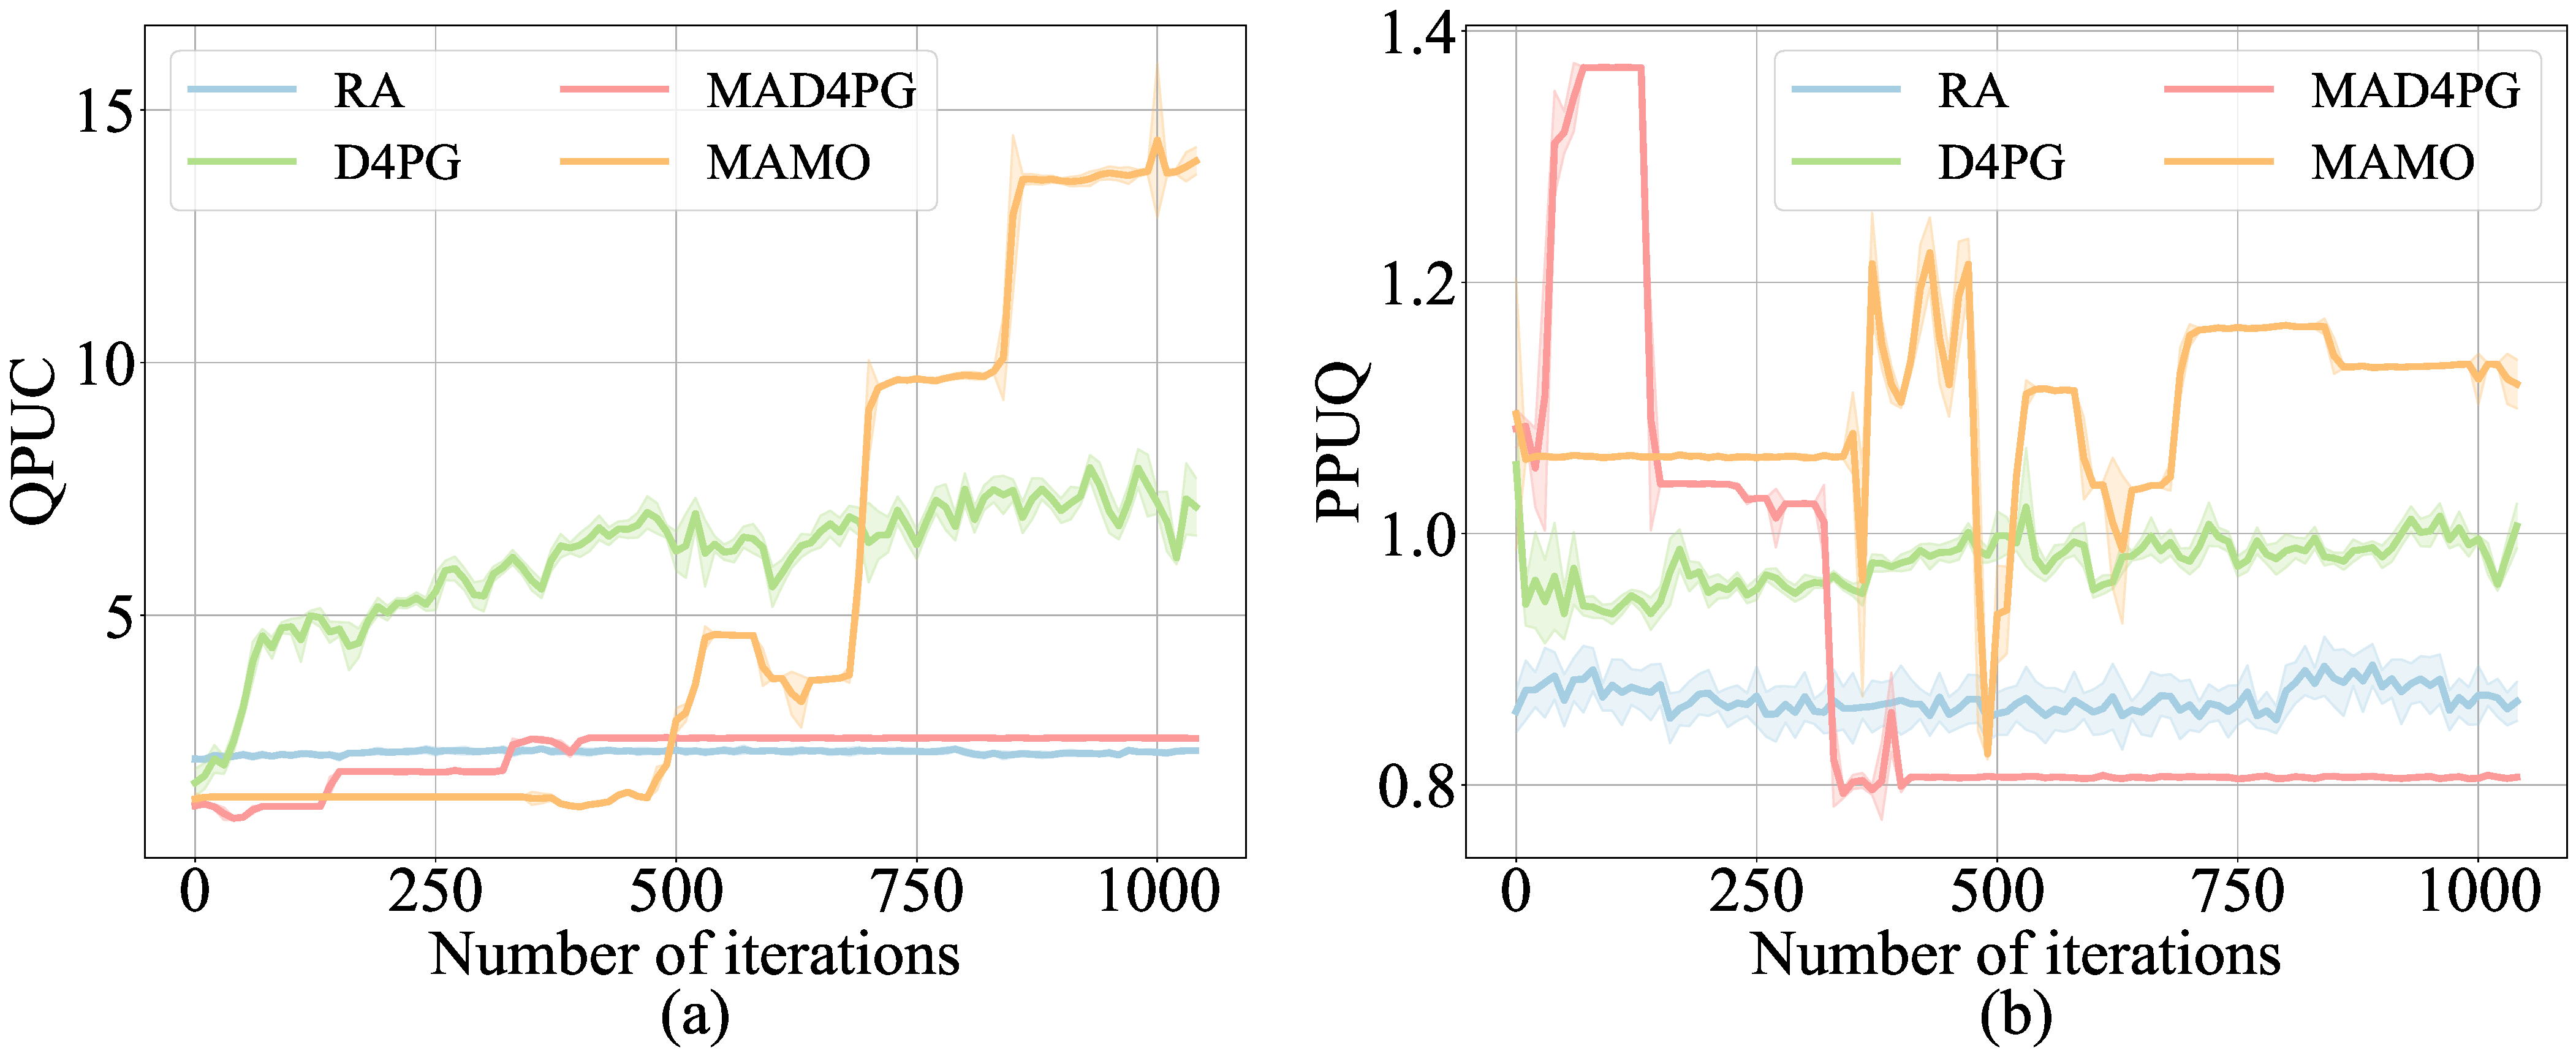
\includegraphics[width=1\columnwidth]{Fig5-3-different-algorithms.pdf}
 \bicaption[算法收敛性比较]{算法收敛性比较。(a)单位开销质量(b)单位质量利润,显示MAMO在收敛后(约850次迭代)与RA、D4PG和MAD4PG相比达到了最高的QPUC和最高的PPUQ}[Convergence comparison]{Convergence comparison. (a) Quality per unit cost (b) Profit per unit quality, which shows MAMO achieves the highest QPUC and the highest PPUQ compared with RA, D4PG, and MAD4PG after convergence (around 850 iterations)}
 \label{fig 5-3}
\end{figure}

\textbf{1) 算法收敛性:}图\ref{fig 5-3}比较了四种算法的收敛性。特别是,图\ref{fig 5-3}(a)和\ref{fig 5-3}(b)分别比较了四种算法的QPUC和PPUQ,其中X轴表示迭代次数,Y轴表示达到的QPUC和PPUQ。QPUC和PPUQ越高,意味着VCPS质量和VCPS 开销的表现越好。如上所述,所提出的MAMO方案在大约850次迭代后达到了最高的QPUC(约13.6)和最高的PPUQ(约1.13)。相比之下,RA、D4PG和MAD4PG分别实现了约2.29、7.34和2.58的QPUC,它们分别实现了约0.87、0.99和0.81的PPUQ。与RA、D4PG和MAD4PG相比,MAMO在QPUC方面分别实现了约494.1\%、85.5\%和428.8\%的改善,在PPUQ方面分别实现了约30.6\%、14.2\%和40.7\%的改善。
值得注意的是,MAMO是唯一一个可以同时改善QPUC和PPUQ的方案。
这显示了MAMO在同时实现QPUC和PPUQ最大化方面的优势。

\begin{figure}[h]
 \centering
 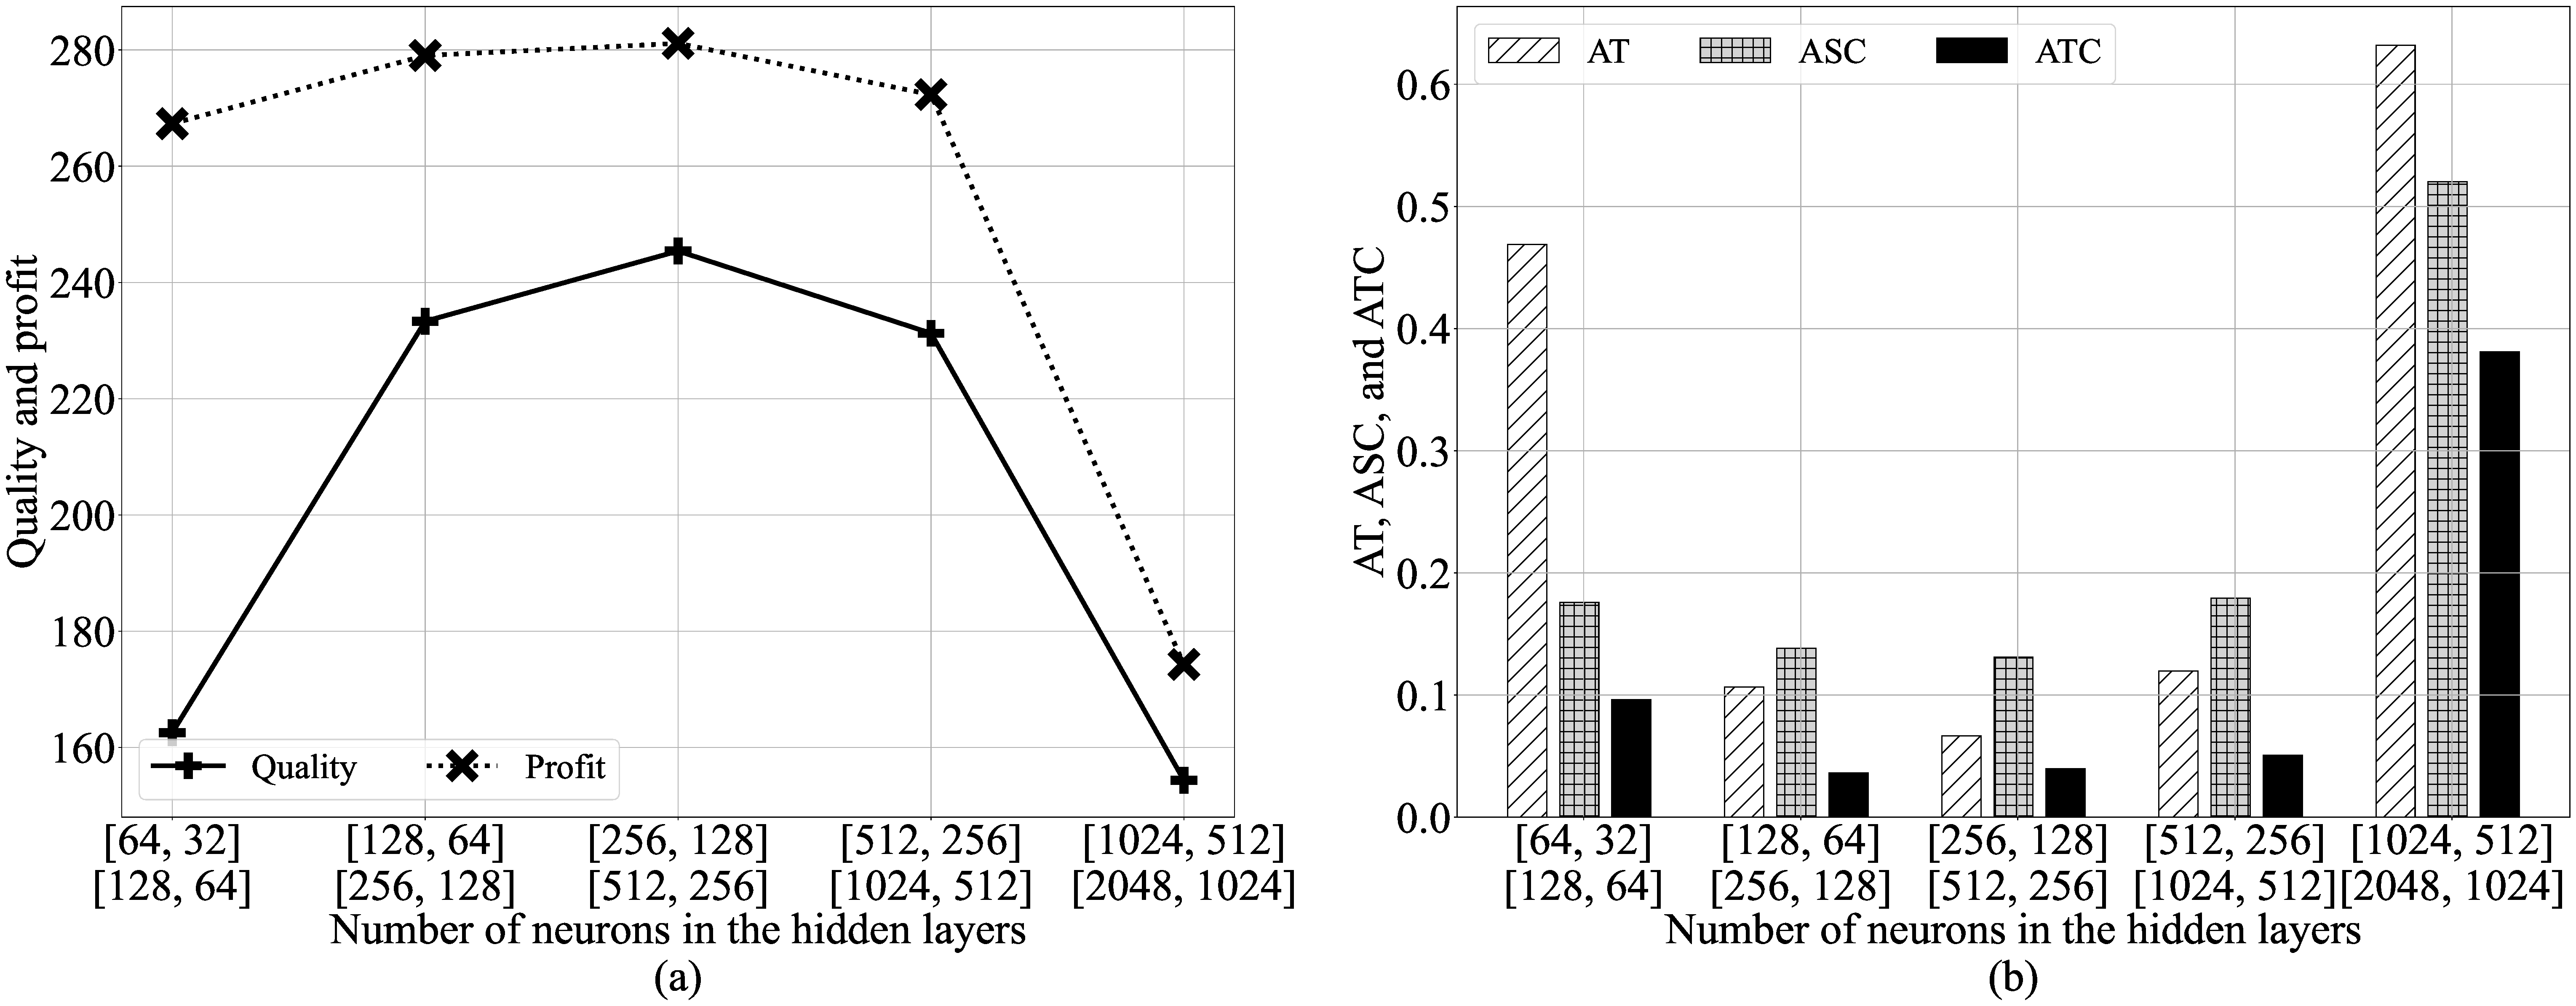
\includegraphics[width=1\columnwidth]{Fig5-4-different-networks.pdf}
 \bicaption[隐藏层中不同数量神经元下MAMO性能比较]{隐藏层中不同数量神经元下MAMO性能比较。(a)单位开销质量(b)单位质量利润}[Performance comparison of MAMO under different numbers of neurons in the hidden layers]{Performance comparison of MAMO under different numbers of neurons in the hidden layers. (a) Quality per unit cost (b) Profit per unit quality}
 \label{fig 5-4}
\end{figure}

\textbf{2) 神经元数量的影响:}
图\ref{fig 5-4}比较了MAMO在不同神经元数量下的性能,其中X轴表示策略网络和评论家网络的两个隐藏层的神经元数量,分别设置为[64, 32] $\sim$ [1024, 512],和[128, 64] $\sim$ [2048, 1024]。如图\ref{fig 5-4}(a)所示,当策略网络和评论家网络的隐藏层的神经元数量被设置为默认设置(即[256, 128]和[512, 256])时,MAMO达到了最高的VCPS质量和最高的VCPS 利润。图\ref{fig 5-4}(b)比较了其他三个指标,包括AT、ASC和ATC。AT、ASC和ATC越低,意味着在信息新鲜度、感知开销和传输开销方面的表现越好。本章注意到,在每个隐藏层的神经元数量设置为默认的情况下,MAMO在最小化AT、ASC和ATC方面取得了最佳性能。

\begin{figure}[h]
 \centering
 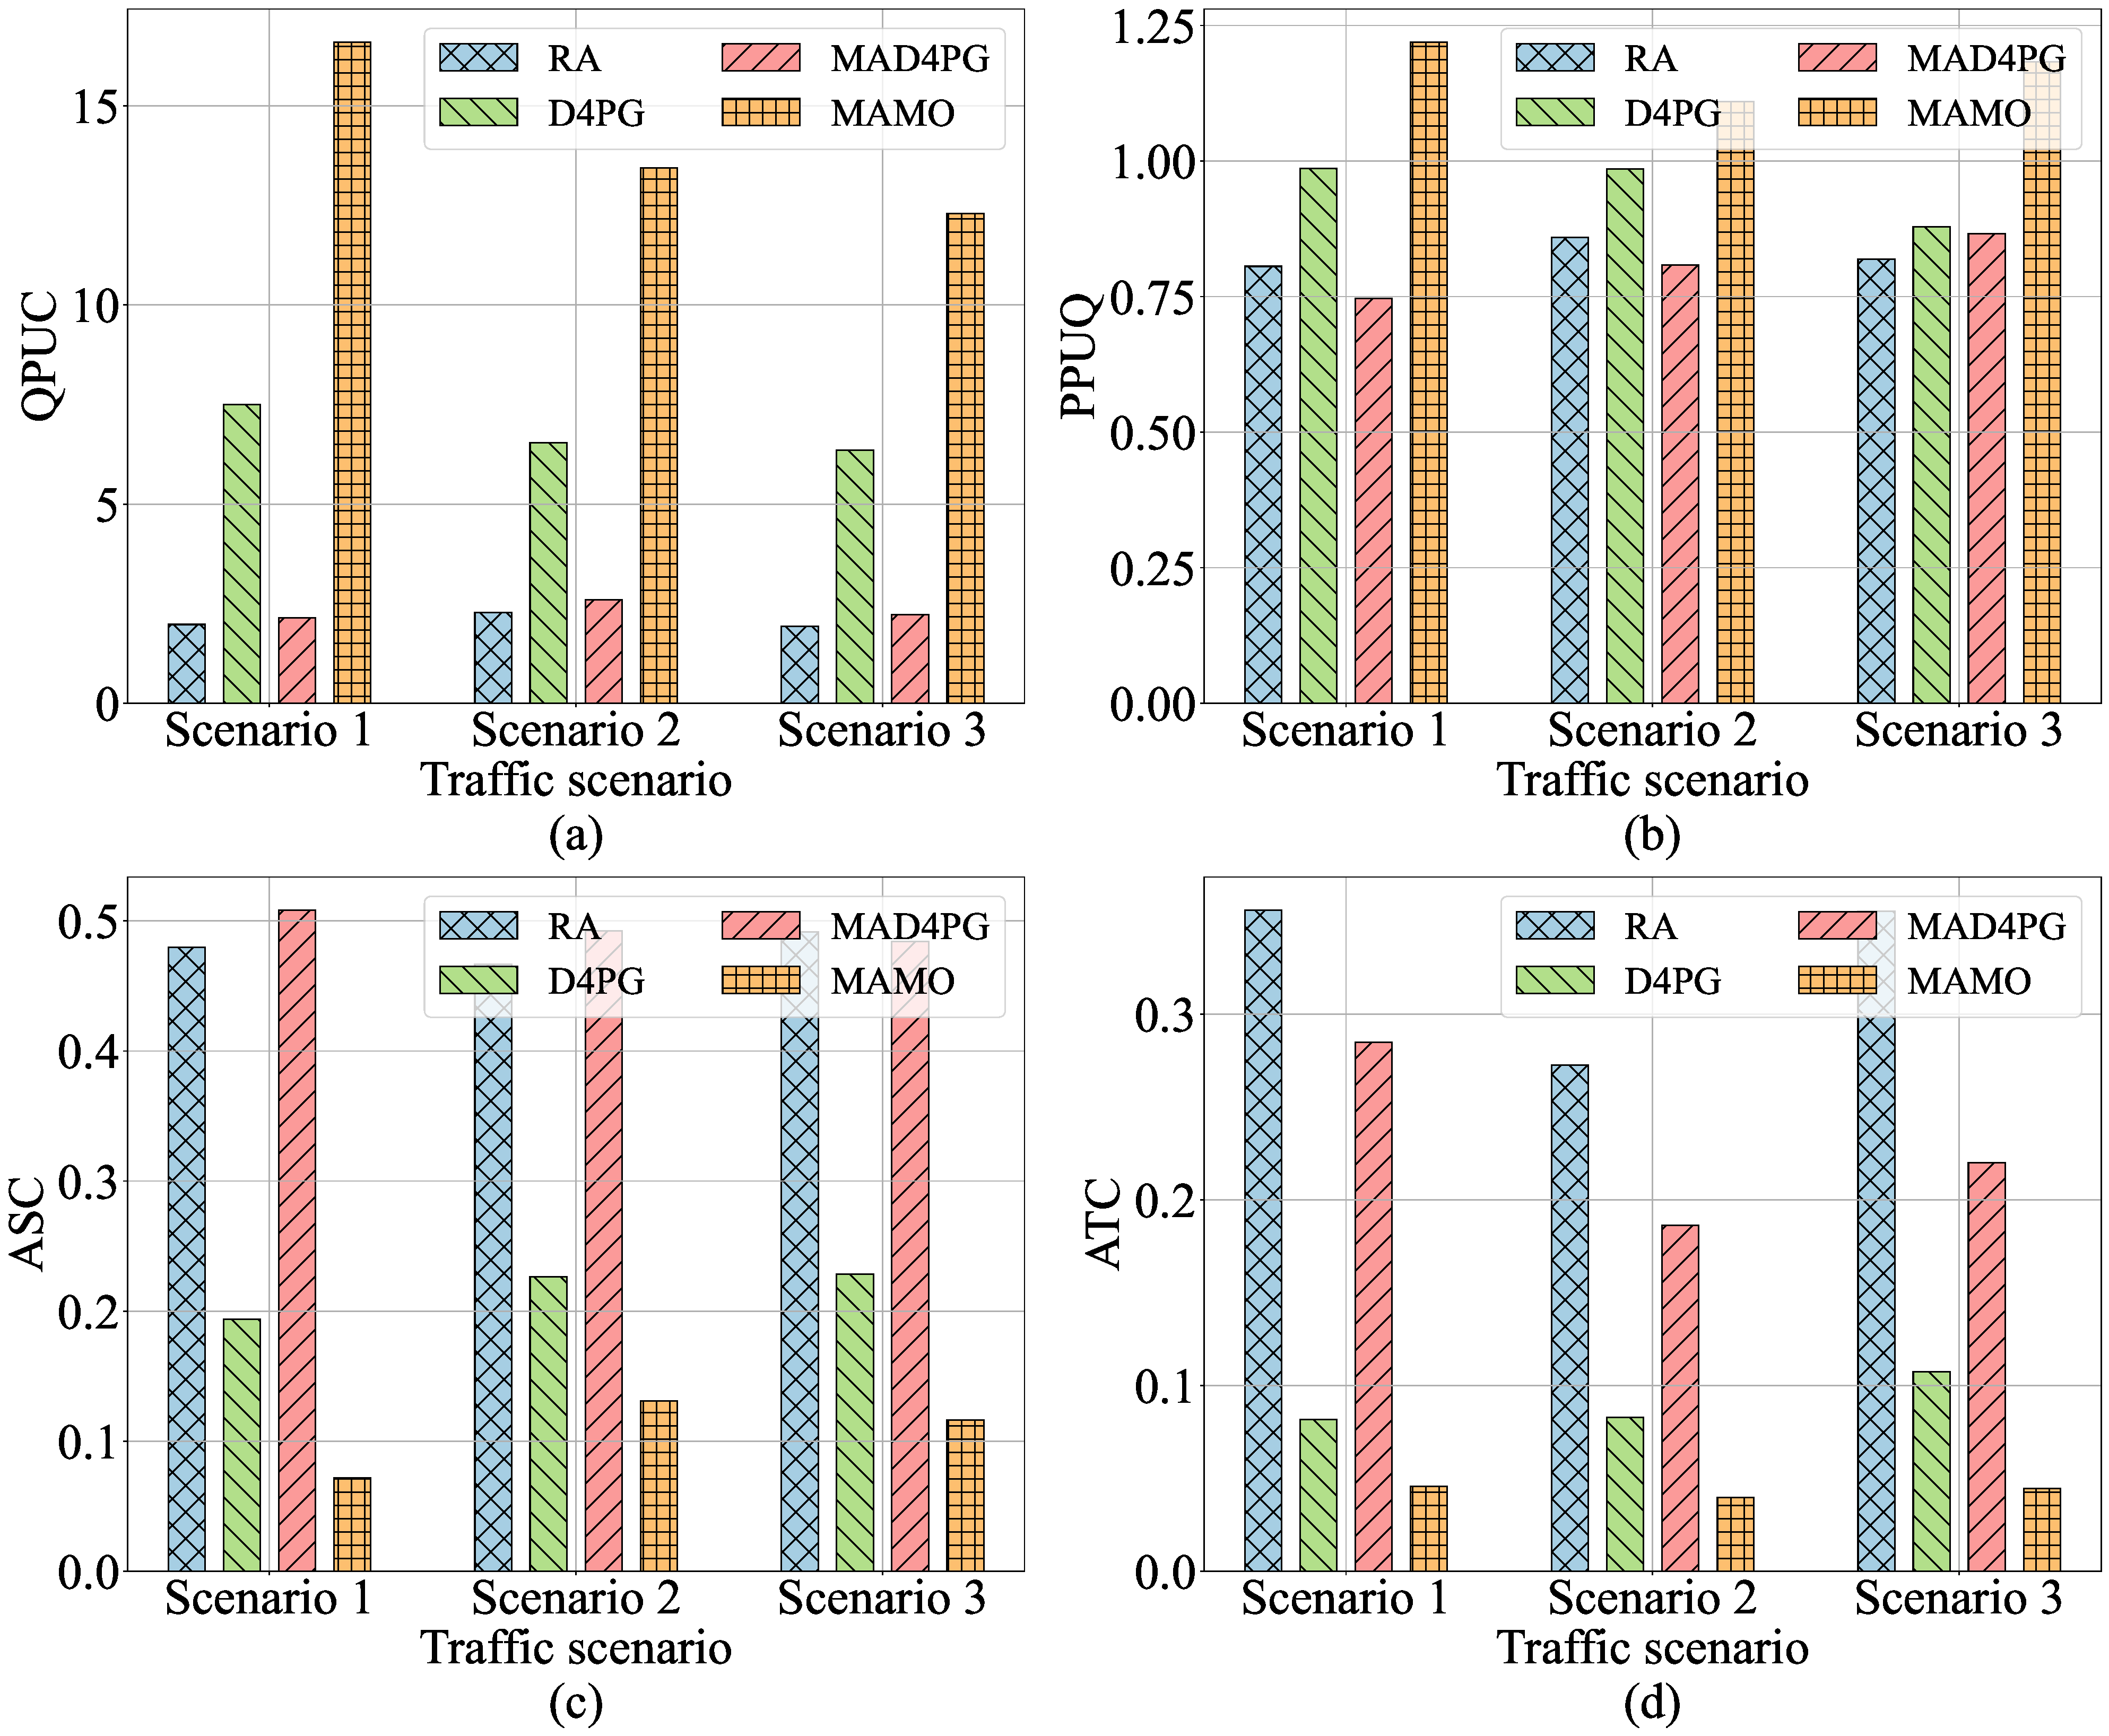
\includegraphics[width=1\columnwidth]{Fig5-5-different-scenarios.pdf}
 \bicaption[不同交通场景下的性能比较]{不同交通场景下的性能比较。(a)单位开销质量(b)单位质量利润(c)平均感知开销(d)平均传输开销}[Performance comparison under different traffic scenarios]{Performance comparison under different traffic scenarios. (a) Quality per unit cost (b) Profit per unit quality (c) Average sensing cost (d) Average transmission cost}
 \label{fig 5-5}
\end{figure}

\textbf{3) 交通情况的影响:}
图\ref{fig 5-5}比较了四种算法在不同交通场景下的性能,其中X轴表示交通场景,在不同的时间和空间中提取了现实的车辆轨迹,即1):2016年11月16日8:00至8:05,中国成都市青羊区1平方公里区域;2):2016年11月16日23:00至23:05,同一区域;3):2016年11月27日8:00至8:05,中国西安碑林区1平方公里区域。图\ref{fig 5-5}(a)比较了四种算法的QPUC。如图所示,MAMO在所有场景下都取得了最高的QPUC。图\ref{fig 5-5}((b)比较了这四种算法的PPUQ。可以预见,MAMO在所有情况下都能达到最高的PPUQ。特别是,与RA、D4PG和MAD4PG相比,提议的MAMO解决方案分别提高了589.0\%、106.7\%和514.8\%的QPUC,并提高了约41.6\%、23.6\%和45.7\%的PPUQ。
图\ref{fig 5-5}(c)比较了这四种算法的ASC。
如上所述,MAMO的ASC低于RA、D4PG和MAD4PG。
这表明MAMO可以通过合作感知信息在车辆间进行合作。
图\ref{fig 5-5}(d)比较了四种算法的ATC。
如图所示,在不同的情况下,MAMO的ATC是最低的。

\begin{figure}[h]
 \centering
 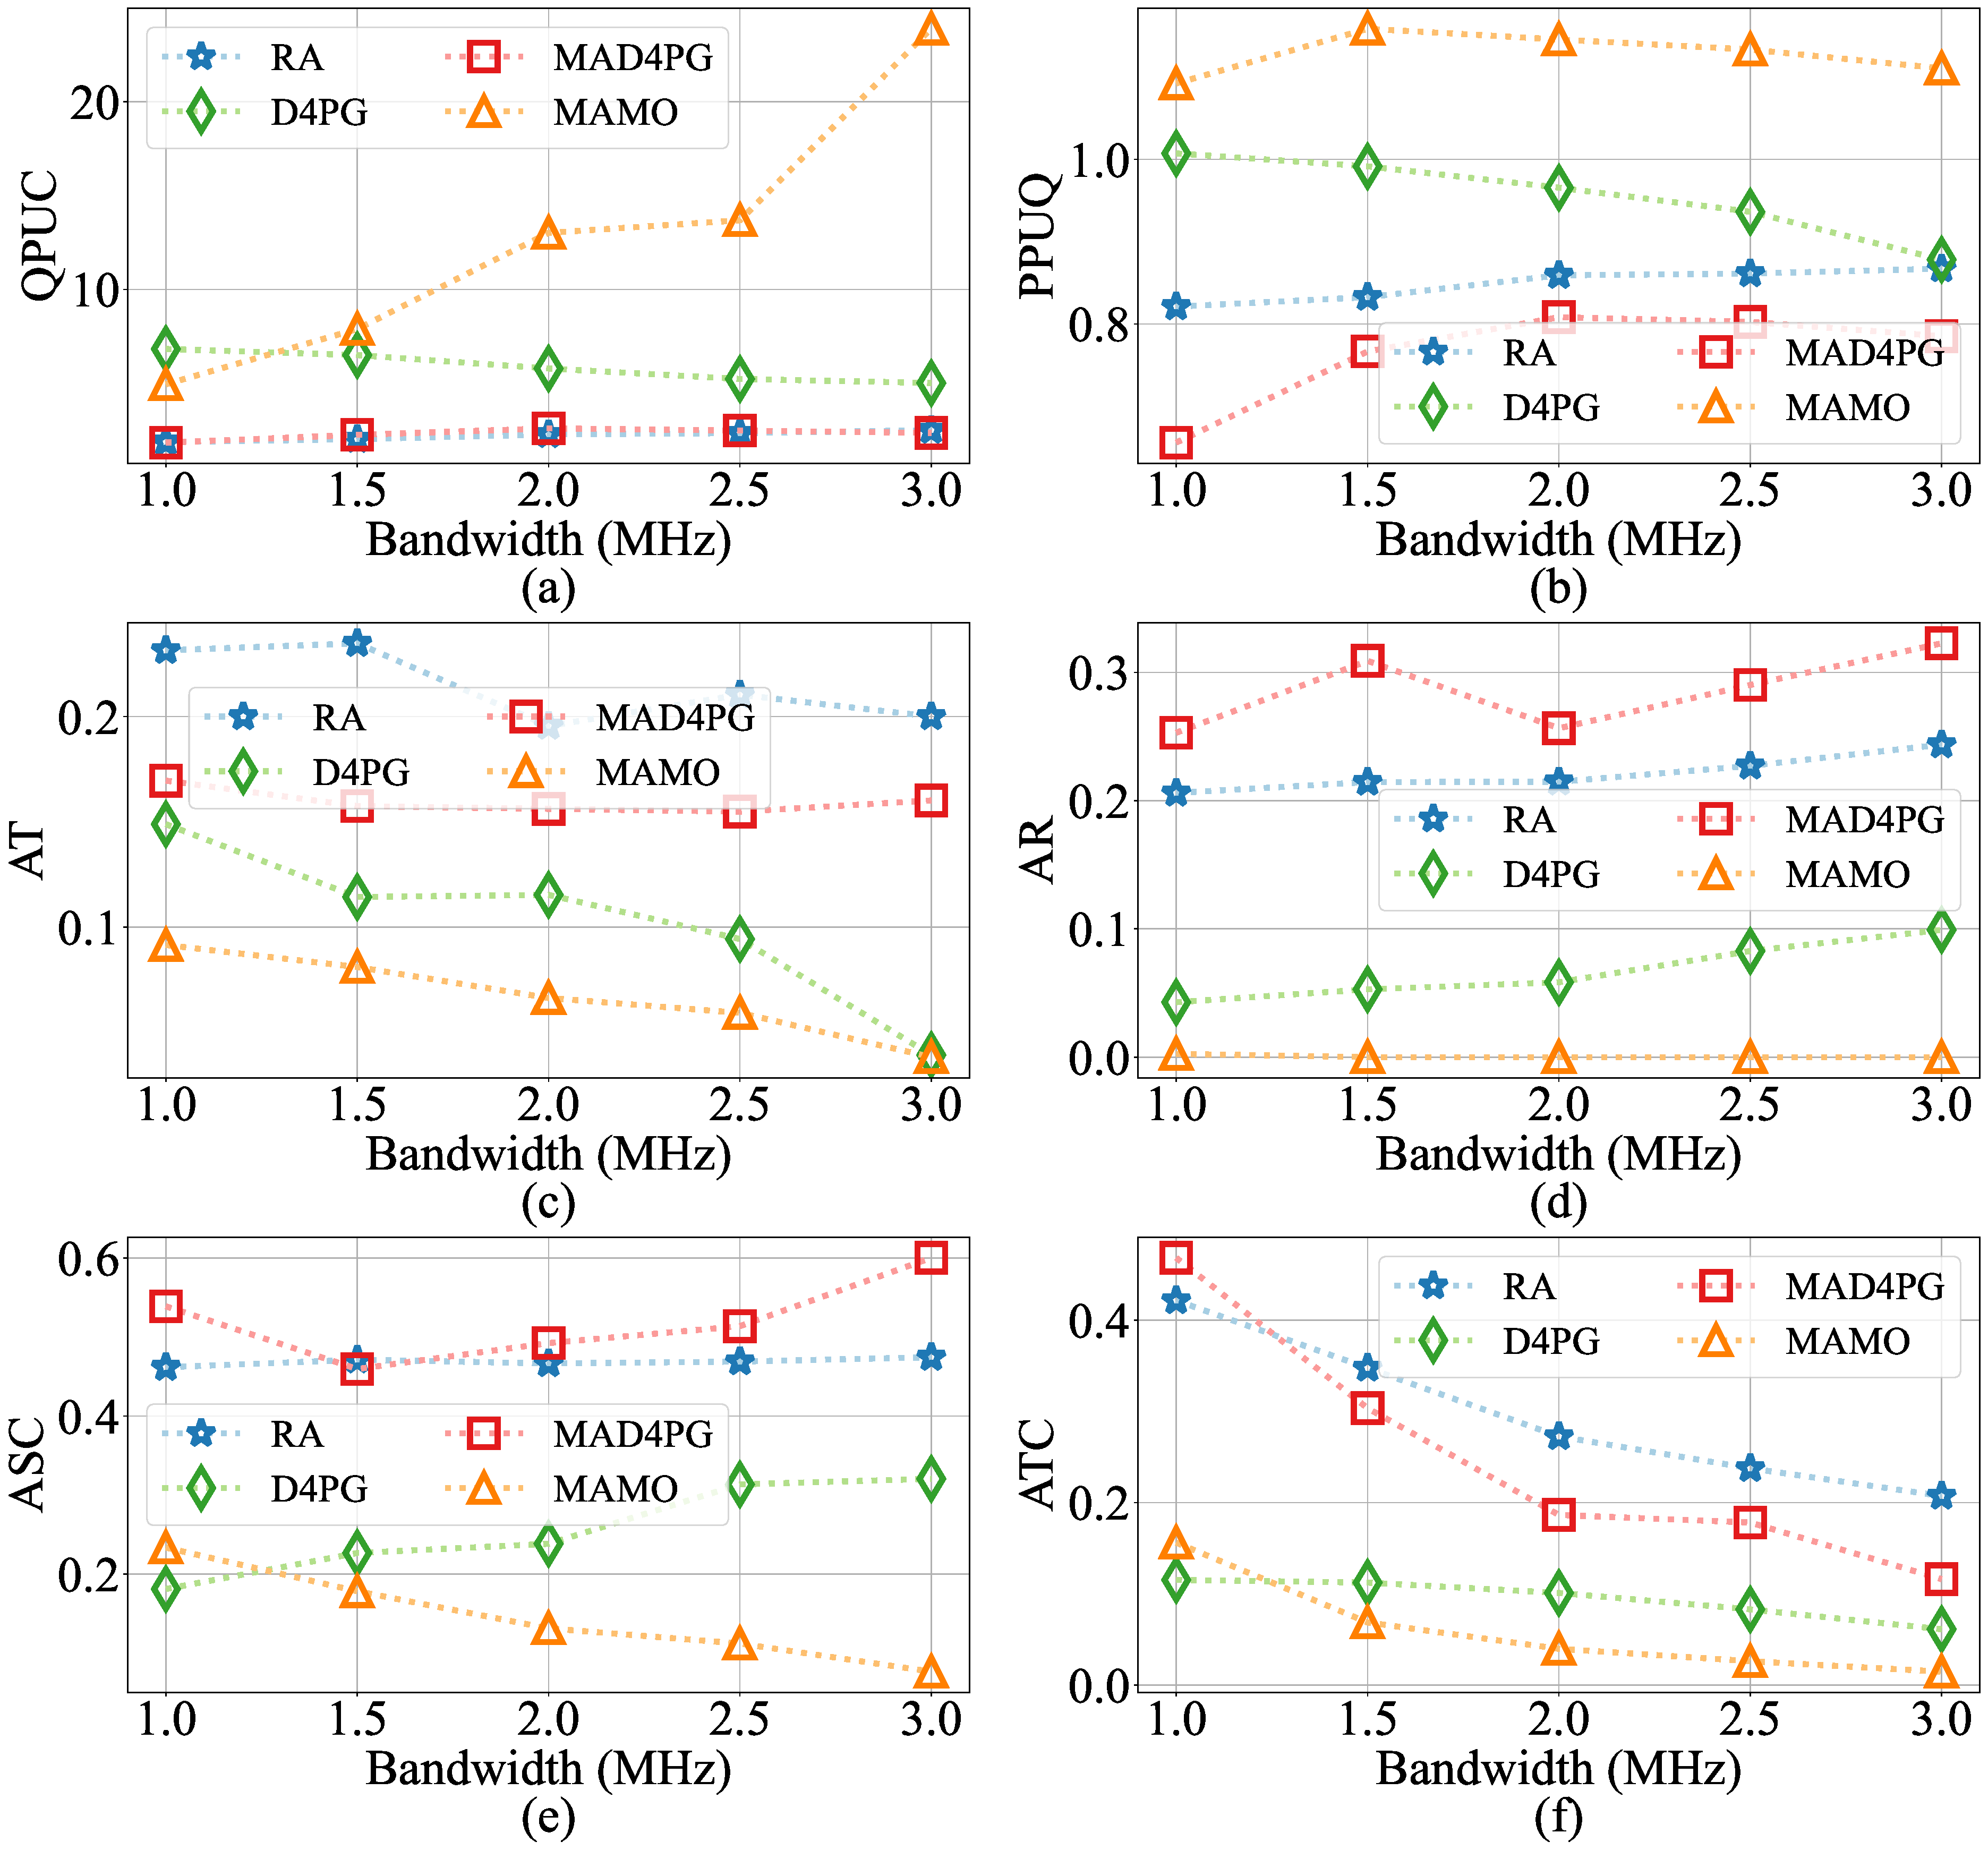
\includegraphics[width=1\columnwidth]{Fig5-6-different-bandwidths.pdf}
 \bicaption[不同V2I带宽下的性能比较]{不同V2I带宽下的性能比较。(a)单位开销质量(b)单位质量利润(c)平均时效性(d)平均冗余度(e)平均感知开销(f)平均传输开销}[Performance comparison under different V2I bandwidths]{Performance comparison under different V2I bandwidths. (a) Quality per unit cost (b) Profit per unit quality (c) Average timeliness (d) Average redundancy (e) Average sensing cost (f) Average transmission cost}
 \label{fig 5-6}
\end{figure}

\textbf{4) V2I带宽的影响:}
图\ref{fig 5-6}比较了四种算法在不同V2I带宽下的性能,其中X轴表示V2I带宽,从1MHz增加到3MHz。较大的V2I带宽代表每辆车分配的V2I带宽可以被扩大。图\ref{fig 5-6}(a)比较了四种算法的QPUC。随着带宽的增加,MAMO的QPUC也相应增加。这是因为在带宽丰富的MAMO中,车辆之间的感应和上传合作更加有效。图\ref{fig 5-6}(b)显示了四种算法的PPUQ,可以进一步证明这一优势。如图所示,MAMO在不同的V2I带宽下实现了最高的PPUQ。特别是,MAMO比RA、D4PG和MAD4PG分别提高了约453.3\%、131.4\%和437.6\%的QPUC,并使PPUQ提高了约33.0\%、18.3\%和48.4\%。
图\ref{fig 5-6}(c)比较了这四种算法的AT。
可以预见,MAMO实现了最低的AT。
可以看出,当带宽从2.5MHz增加到3MHz时,MAMO和D4PG的性能差异很小。
这是因为随着带宽的增加,数字孪生的及时性改善是有限的。
图\ref{fig 5-6}(d) 比较了四种算法的AR。
AR越低意味着协同感知和上传的性能越好,MAMO有望实现最低的AR。
图\ref{fig 5-6}(e)和\ref{fig 5-6}(f)分别比较了四种算法的ASC和ATC。
可以看出,当带宽增加时,这四种算法的ATC都会下降。
原因是,当带宽增加时,信息上传时间减少,导致传输开销降低。
正如预期的那样,MAMO的ASC和ATC在大多数情况下保持在最低水平。

\begin{figure}[h]
 \centering
 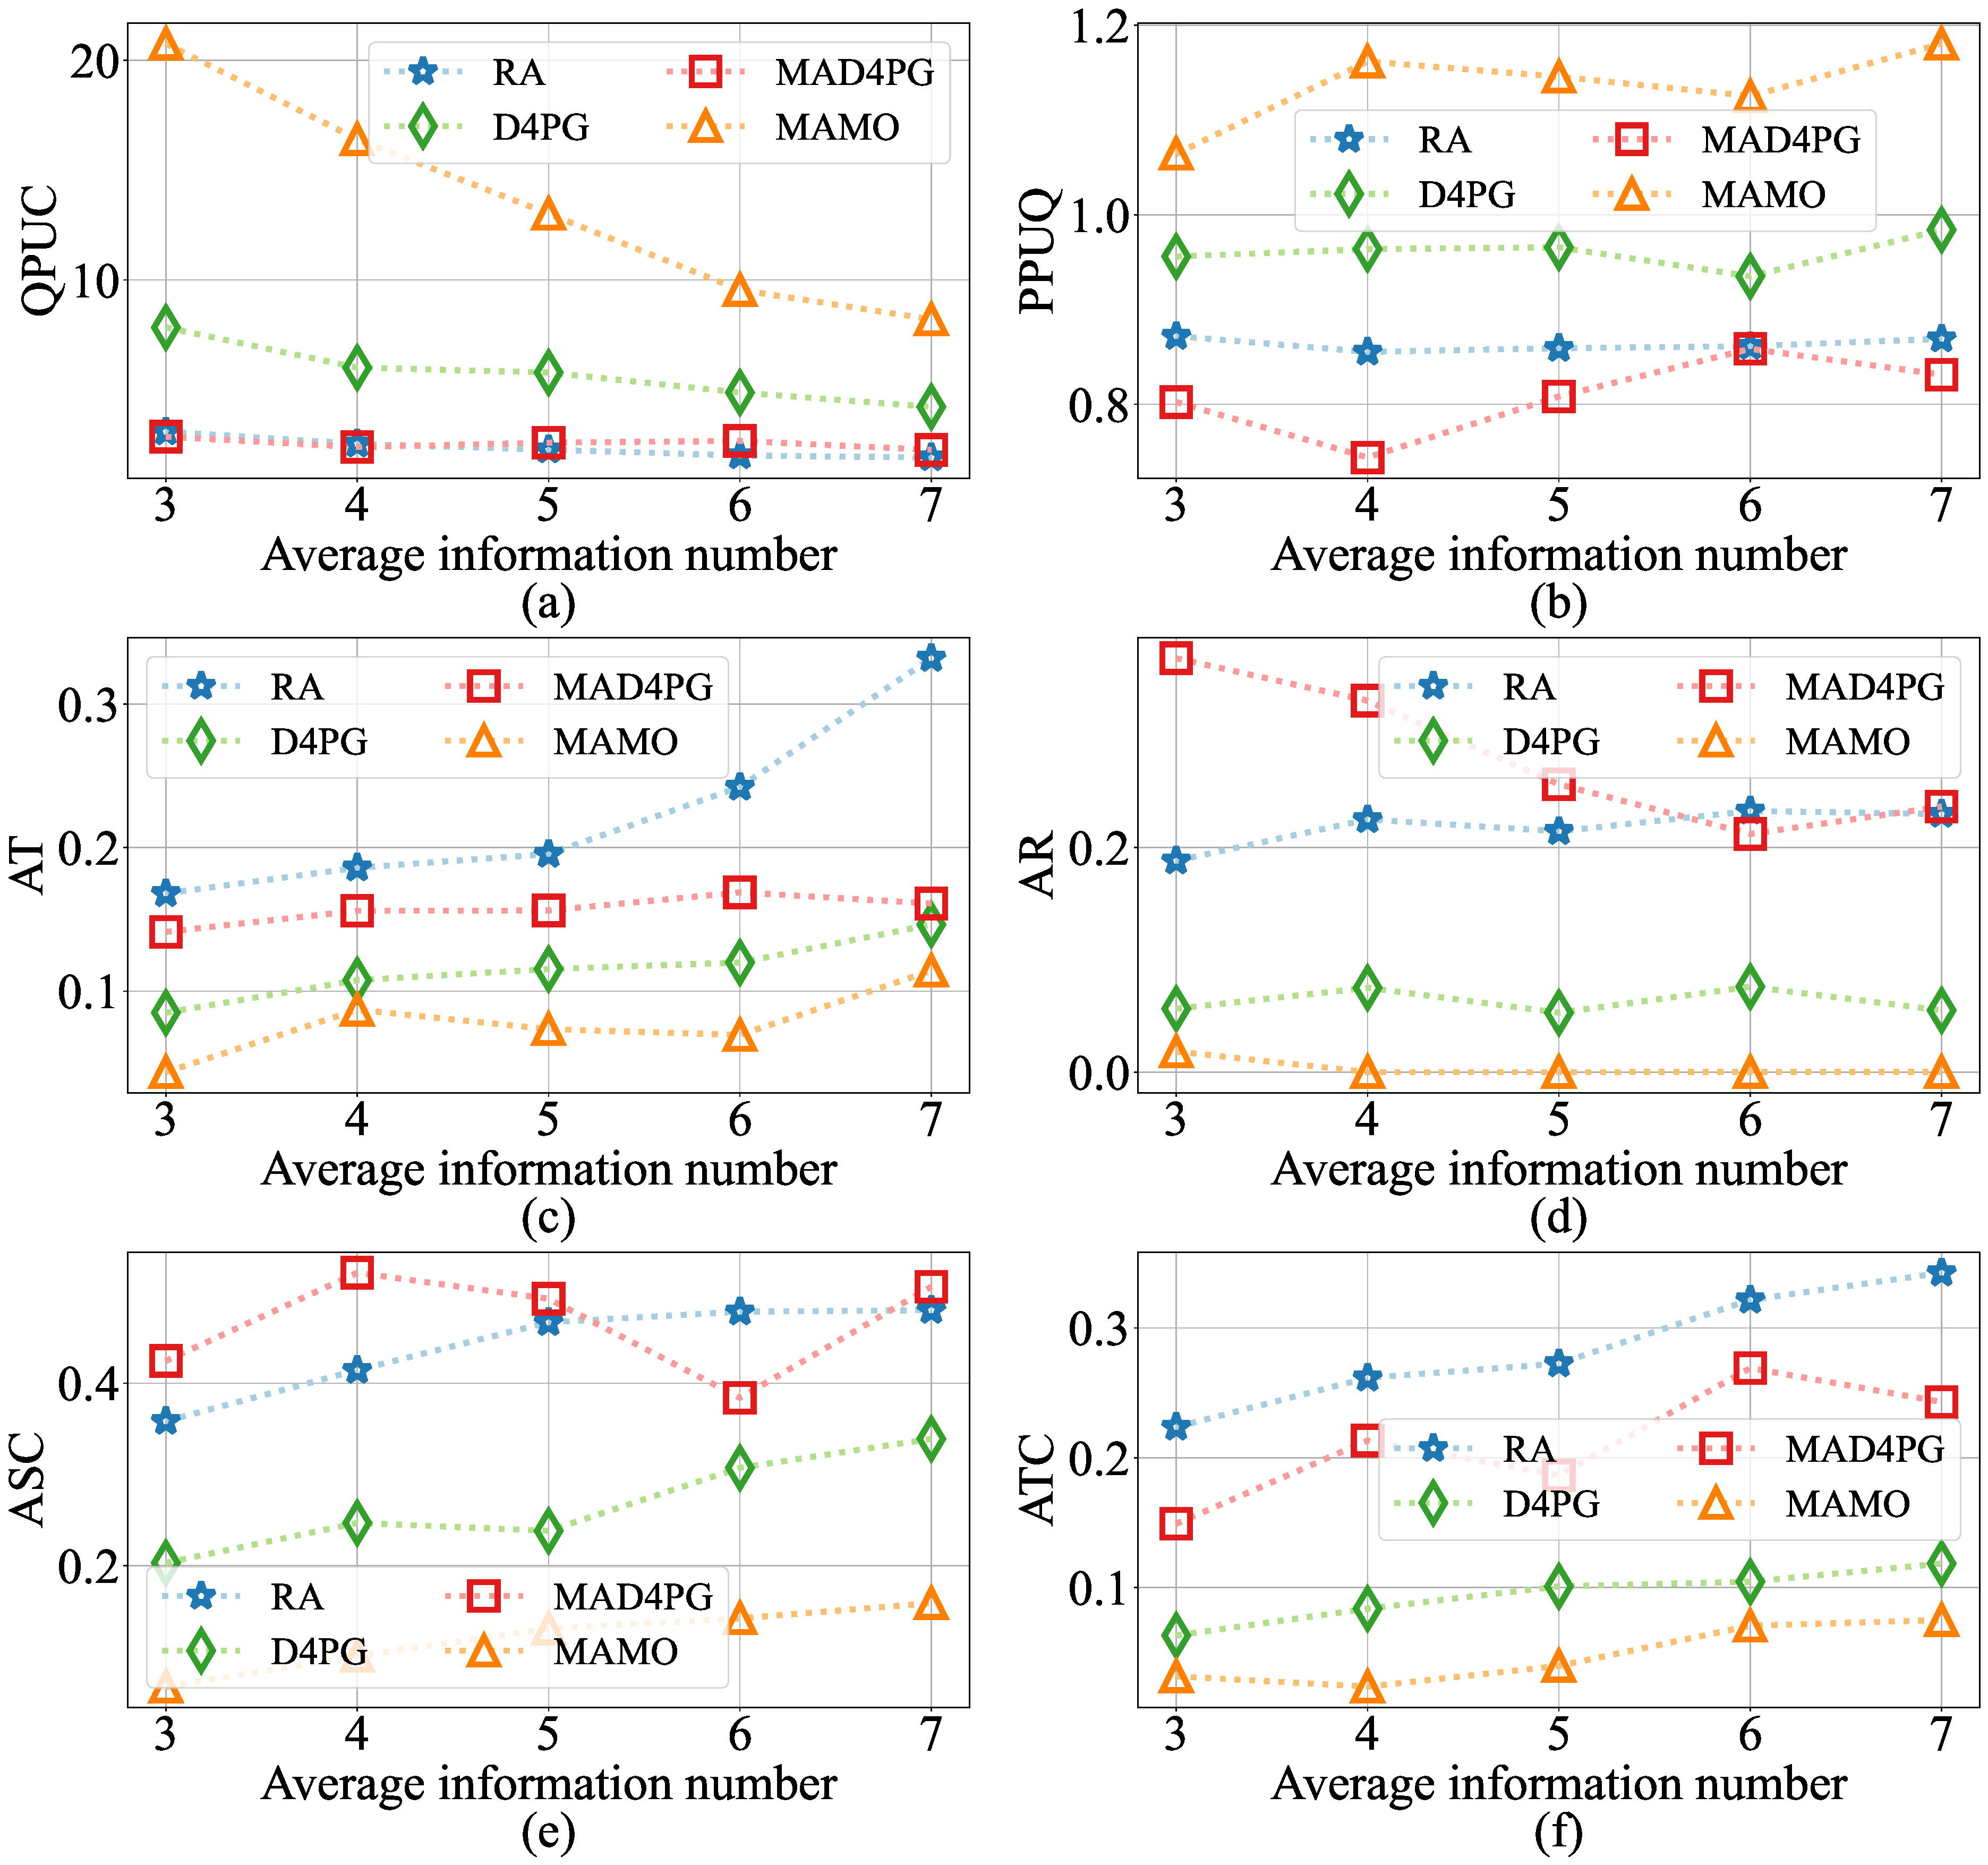
\includegraphics[width=1\columnwidth]{Fig5-7-different-numbers.pdf}
 \bicaption[不同数字孪生需求下的性能比较]{不同数字孪生需求下的性能比较。(a)单位开销质量(b)单位质量利润(c)平均时效性(d)平均冗余度(e)平均感知开销(f)平均传输开销}[Performance comparison under different digit twin requirements]{Performance comparison under different digit twin requirements. (a) Quality per unit cost (b) Profit per unit quality (c) Average timeliness (d) Average redundancy (e) Average sensing cost (f) Average transmission cost}
 \label{fig 5-7}
\end{figure}

\textbf{5) 数字孪生需求的影响:}
图\ref{fig 5-7}比较了四种算法在不同数字孪生需求下的性能,其中X轴表示数字孪生体所需信息的平均数量从3增加到7。数字孪生所需信息的平均数越大,说明车辆的感知和上传工作负荷越大。图\ref{fig 5-7}(a) 比较了四种算法的QPUC。随着平均所需信息数的增加,四种算法的QPUC也相应减少。如前所述,MAMO在所有情况下都保持最高的QPUC。图\ref{fig 5-7}(b) 比较了四种算法的PPUQ。正如预期的那样,MAMO在所有情况下都取得了最高的PPUQ。特别是,MAMO的QPUC比RA、D4PG和MAD4PG分别高出458.7\%、130.6\%和426.2\%,而MAMO的PPUQ比RA、D4PG和MAD4PG分别高出31.5\%、18.2\%和40.7\%。
图\ref{fig 5-7}(c)比较了四种算法的AT。
正如预期的那样,MAMO在AT方面取得了最佳性能。
图\ref{fig 5-7}(d)比较了四种算法的AR,表明MAMO可以在所有情况下实现最低的AR。
图\ref{fig 5-7}(e)和\ref{fig 5-7}(f)分别比较了四个算法的ASC和ATC。
本章注意到,当平均信息数增加时,四种算法的ASC和ATC都会增加。
原因是面向车载边缘计算的数字孪生需要的平均信息量增加,导致车辆感应和传输开销提高。

\section{本章小结}\label{section 5-7}

本章提出了车载信息物理融合架构,其中基于分布式感知与V2I协同上传构建车联网要素的数字孪生。
具体地,在信息融合的基础上,车辆数字孪生被建模,并被进一步利用来形成边缘节点的逻辑视图并反映物理车联网环境。
分布式感知模型是基于多类M/G/1优先级队列得出的,V2I协同上传模型是基于信道衰减分布和SNR阈值得出的。
在此基础上,设计了两个指标QDT和CDT,以衡量在边缘节点建模的数字孪生的质量和开销,并制定了一个双目标问题,通过协同感知和上传,使VCPS质量最大化,VCPS 开销最小化。
此外,还提出了一个基于多智能体多目标深度强化学习的解决方案,其中采用了一个决斗评论家网络,根据状态价值和动作优势来评估智能体动作。
最后,进行了全面的性能评估,证明了所提方案的优越性。